\documentclass[a4paper,12pt,oneside]{report}
\usepackage[T1]{fontenc}
\usepackage{setspace}
\usepackage[utf8]{inputenc} 
\usepackage[english]{babel}
\usepackage{url}
\usepackage{tikz}
\usepackage{layaureo}
\usepackage[english]{varioref}
\usepackage{mathtools}
\usepackage{siunitx}
\usepackage{amsfonts}
\usepackage{amsmath}
\usepackage{amssymb}
\usepackage[section]{placeins}
\usepackage{microtype}
\usepackage{booktabs}
\usepackage{svg}
\usepackage[font=small,labelfont=bf]{caption}
\usepackage{subfig}
\usepackage{appendix}
\usepackage{fancyhdr}
\usepackage{graphicx}
\usepackage{xcolor}
\usepackage[autostyle,italian=guillemets]{csquotes}
\usepackage{listings,xcolor}
\addtolength{\textheight}{1cm}
\DeclareMathOperator{\Tr}{Tr}
\usetikzlibrary{decorations.text}
\usetikzlibrary{arrows.meta}
\tikzset{>={Latex[width=2mm,length=2mm]}}
\renewcommand{\chaptermark}[1]{\markboth{#1}{#1}}
\fancypagestyle{styletoc}{
  \fancyhf{}
  \fancyhead[R]{\thepage}
  \fancyhead[L]{CONTENTS}
}
\fancypagestyle{stylenor}{
\fancyhf{}
\fancyhead[R]{\thepage}
\fancyhead[L]{\scshape{\chaptername} \thechapter\ --\ \leftmark}
}
\newlength{\mylen}
\setbox1=\hbox{$\bullet$}\setbox2=\hbox{\tiny$\bullet$}
\setlength{\mylen}{\dimexpr0.5\ht1-0.5\ht2}
\renewcommand\labelitemi{\raisebox{\mylen}{\tiny$\bullet$}}
\onehalfspacing
\setcounter{secnumdepth}{3}
\setcounter{tocdepth}{3}
%\usepackage[backend=biber,style=numeric-comp]{biblatex}
\DeclarePairedDelimiter{\abs}{\lvert}{\rvert}
\DeclarePairedDelimiter{\norma}{\lVert}{\rVert}
%\addbibresource{Bibliografia.bib}
\graphicspath{{./Images/}}
\usepackage{hyperref}
\hypersetup{hidelinks}
%\pagestyle{headings}
\newcommand{\Hline}{\specialrule{.1em}{0em}{0em}}
\begin{document}
\begin{titlepage}

\begin{figure}
\centering

\includegraphics[scale=0.25]{sigillo2}
\end{figure}

\begin{center}
\LARGE{\textbf{Università degli Studi di Trento\\ Department of Industrial Engineering}}\\
\vspace{10mm}
\Large{Master Degree in\\ Mechatronics Engineering}\\
\vspace{7mm}
\uppercase{Final Dissertation}
\vspace{7mm}\\
\huge{Titolo}
\end{center}

\vspace{8mm}
\begin{flushleft}
\large{\textbf{Supervisor:}\\ Daniele Bortoluzzi}\\
\vspace{5mm}
\large{\textbf{Co-supervisor:}\\ Edoardo Dalla Ricca}\\
\vspace{5mm}
\large{\textbf{Student:}\\ Simone Manfredi 239337}\\
\end{flushleft}

\vspace{15mm}
\begin{center}
\Large{Academic Year 2023/2024}
\end{center}

\end{titlepage}

\newpage

\begin{abstract}


\end{abstract}

\newpage
\pagenumbering{roman}
\addcontentsline{toc}{chapter}{Contents}
\tableofcontents
\pagestyle{styletoc}
\chapter*{Introduction}
\pagestyle{stylenor}
\addcontentsline{toc}{chapter}{Introduction}
We live in a society overwhelmed by such technology, autonomous systems, industrial manipulators, AI and, very soon, services' humanoid robots, that we forget to look up in the sky. Most of the major progress in robotics and the scientific field is done in space, where human curiosity is pushing our abilities beyond any imaginable scenario.\\
This thesis was born due to my curiosity in the field of robotics merged with the need to face space and modern problems, such as the berthing and docking of external objects by a manipulator or the tumbling of a spinning satellite. This dissertation aims to analyse the dynamic of a space manipulator after the impact with an external satellite/meteorite to retrieve its kinetic properties before the impact.
\clearpage
\pagenumbering{arabic}
\chapter{Space Manipulators: an Overview}
Space Robotics is important to human's overall ability to explore or operate in space. Autonomous systems can reduce the cognitive load on humans and improve human and systems' safety.\\
Space robots can be split into two main categories: orbital robots and planetary robots. The formers can be used for repairing satellites, assembling large space telescopes, capturing and returning asteroids, etc; the latter play a key role in surveying, observations, extraction, working on planetary surfaces for subsequential human arrival, etc.\\
Furthermore, spacecraft are classified as space robots when two attributes are satisfied: locomotion and autonomy. Depending on its application, a space robot is designed to possess locomotion to manipulate, grip, rove, drill and/or sample; at the same time, it is expected to possess varying levels of autonomy, ranging from teleoperation by humans to fully autonomous operation by the robot itself [3].\\
Another classification of robotic devices in space could be represented by mobile robots, flying robots, and manipulators. Manipulators are used on board spacecraft (Space Shuttle) or space stations [5].
According to [1], a very loose definition calls every unmanned space probe a robotic spacecraft, referring to the challenges of largely autonomous operation in a complex mission. But even discarding this and focussing on space robotics elements in a more narrow sense (systems involving arms for manipulation or some kind of locomotion device for mobility and having the flexibility to perform varying tasks), there is a wide array of uses in the scope of space missions, giving rise to challenging problems and ingenious solution.\\
Robots and manipulators in space are designed to perform the following operations:
\begin{itemize}
\item capture
\item maneuvring
\item berthing/unberthing
\item support of Extra-Vehicular-Activities (EVA)
\item positioning and release
\end{itemize}
One of the most important features of all robots deployed in space is their flexibility. Robots and manipulators used in space are built out of light materials, and very often, their links deflect.\\
There are quite a number of on-orbit applications requiring advanced robotics capabilities, which
are envisaged to take place in the 2025-2035 timeframe. The operators for these missions may
range from space administrations to national governments to businesses. The following mission
foci are envisaged: space debris removal, rescue mission, planned orbit raising,
inspection/support to deployment, deployment/assembly aid, repair, refuelling and orbit
maintenance, mission evolution/adaptation, lifetime extension, and re/de-orbiting. The
International Space Station (ISS) continues to represent an excellent opportunity for scientific
experiments to be conducted in space amid the unique characteristics, constraints and pressures that the environment brings [3].\\
But what is so special about a space robot? In many ways, robot systems for space applications are very different from the more familiar terrestrial robots, be they industrial robots in production automation or the newer kind of "service robots". One of the main and simplest differences is the high development and manufacturing costs and the missing "economy of scale" due to the experimental prototype nature of these developments.\\
This thesis will investigate space manipulators' dynamics, whose tasks involve berthing and docking satellites or managing tumbling meteorites; thus, a historical summary of their evolution and the actual state-of-art of this field will be briefly exposed.
\newpage
\section{Historical background}
The first robot used in space was the Remote Manipulator System (RMS), also called \textit{Canadarm}, developed by the Canadian Space Agency and mounted on the Space Shuttle. This robot was used for the first time on 12th November 1981 in the Columbia Shuttle and it was retired in July 2011. It is 15 meters long and has three hinged joints for pitch and three others for yaw and roll, which makes a total of six degrees of freedom (DOF).\\
There were numerous problems related to the use of the RMS in space. One of the most important was related to its positioning: since it is built out of light materials to minimise the launch cost, its links deflect substantially. When the arm is accelerated and stopped, large vibrations occur.\\
There are two main methods of improving the positioning accuracy of the RMS: passive and active. The passive methods focus on redesigning the manipulator and applying different materials. The active ones refer to a preshape input and to the usage of position, velocity or force feedback.\\
Eventually, some lessons have been learnt during the RMS' lifetime: the speed of manipulation should be drastically improved; the positioning accuracy is one of the most important issues in day-to-day operations; the new manipulators should be designed to include passive vibration control capabilities; active vibration control should be added in order to improve the positioning accuracy and shorten the settling time; the force loop could add significantly to the capabilities of the manipulator [5].\\
It is interesting to note that the actuators are not powerful enough to lift even the weight of the arm itself when on Earth. The Canadarm has been used for over 100 operations and is normally used for repairing, retrieving, and deploying satellites; assisting humans during extravehicular activi- ties; and for remote inspection tasks [6].\\
Another early mission including a robotic arm in space was the MIR space station. This Soviet Union/Russian space station was the first modular space station and was in operation from 1986 to 2001. MIR was a microgravity research laboratory which conducted research in biology, astronomy, meteorology, and physics, to name a few. Four of the modules were equipped with the Lyappa robotic arm used for assembling the modules of the space station.\\
In 1997 the National Space Development Agency of Japan (NASDA) launched the Engineering Test Satellite No. 7 (ETS-VII), the first ever satellite to be equipped with a robotic arm. The ETS-VII performed several successful docking operations using the manipulator arm. The main objectives of the project were performance evaluation of a satellite-mounted robotic system; coordinated control of the satellite attitude and robot arm; teleoperation of the robot arm; demonstration of in-orbit satellite servicing.\\
The project demonstrated the successful execution of experiments which gained insight into operations such as docking, fuel transfer, assembling, and berthing. Several successful docking operations were performed with the chaser and target satellite.\\
The Japanese also developed a robotic arm which was mounted on the Japanese Experiment Module at the International Space Station (ISS), the JEMRMS, in March 2008. The Small Fine Arm (SFA) was added in July 2009 (see Section~\ref{state_of_art}).\\
A larger and more advanced version of the SRMS arm is the MSS arm (Mobile Servicing System), which is mounted on the International Space Station. The MSS arm consists of a mobile base, a more advanced version of the Canadarm, called the \textit{Canadarm2}, or SSRMS, and dexterous manipulator hand [6]. It has seven DOF, unlike the RMS, making it a redundant manipulator to avoid singularities in some specific but important positions. Its properties will be discussed in the next Section. [5]\\
In March 2008 the last part of the Mobile Servicing System was added to the International Space Station. The Canada Hand, or the Special Purpose Dexterous Manipulator (SPDM), is a two-armed robot but is often referred to as a hand be- cause it can be attached to the Canadarm2 robotic arm and taken to any location on the space station [6].\\
The last manipulator in space was launched in July 2021: the Europian Robotic Arm (ERA) serves as main manipulator on the Russian part of the Space Station.\\
Clearly, the usage of manipulator in space involves recent activities, hence a lot of research and experiments are still in development. This research field offers numerous starting points in analysis and technologic progress.
\newpage
\section{Main characteristics}
Orbiting robotic systems consist of a free-floating base, typically a satellite or a space station, with a robotic manipulator attached to it.\\
The main difference between space manipulators and Earth-based robots is the lack of a fixed base on which the robot is mounted.\\
Depending on whether or not actuation is utilized to control the spacecraft position and orientation, we can divide these systems into \textit{free-flying} and \textit{free-floating} space manipulators. \\
In a free-flying robotic system the position and orientation of the base, in this case the spacecraft, is actively controlled by the spacecraft’s actuators. This allows to completely control both the base configuration and the manipulator arm.\\ 
Due to the dynamic coupling between the manipulator and the spacecraft, the motion of the manipulator arm will constantly affect the motion of the base. The main concern with these systems is therefore the excessive fuel consumption required to compensate for the dynamic coupling between the manipulator and the base while maintaining a constant base attitude [6].\\
This mode is employed during the final approach of a manipulator to its target, so that the target is within the manipulator workspace [2].\\
A free-floating robotic system, on the other hand, does not use spacecraft actuation to compensate for the manipulator motion. The spacecraft motion is therefore not controlled directly, but arises as a result of the dynamic coupling between the manipulator and the base. In this case one can either choose not to control the spacecraft motion at all (as it has been done in this work), or to use the manipulator arm to obtain the required motion also for the spacecraft. In many cases it is necessary to generate a manipulator motion which guarantees that the spacecraft orientation remains almost constant so that antennas and other instruments point in the right direction [6].\\
In this mode, the spacecraft attitude is controlled actively with momentum control devices (MCD), such as reaction wheels or momentum gyros, while the system CoM does not translate. The free-floating or the partial free-floating modes are preferred during grasping, since they eliminate sudden motions due to thrusters, and conserve propellant and power [2].\\
Even though space exploration is challenging compared to Earth-based systems, space manipulator design also benefits from the free-fall environment in some areas. It is, for example, possible to construct robots with extremely high redundancy and with several joints. This type of robots, are able to support their own weight in space due to the small gravitational forces. On Earth, however, such robots would collapse due to their own weight when the number of joints becomes too large. This allows for more redundant robots in space than on Earth, and also more fault tolerant robots because the robots can continue operation even after several joint failures. Similarly, the free-fall environment allows for effective control with very small actuators. In fact, most space manipulators are able to handle very high payloads in space, while they cannot even withstand the weight of the manipulator arm itself if they were to be placed in the Earth’s gravity field [6].\\

To execute on-orbit tasks being inaccessible to, or too dangerous for humans, robotic on-orbit servicing (OOS) can be employed, with tasks to be performed by space manipulator systems (SMSs), also called chasers or servicers in the literature. An SMS consists of a satellite base equipped with one or more robotic manipulators (arms) with grappling devices on them and driven by a vision system which allows them to capture a target (client) satellite, or another object. An SMS also can be a large servicing manipulator mounted on a space facility.\\
Targets for capture may be cooperative, i.e., a stable and safe target due to its operational Attitude and Orbit Control Subsystem (AOCS), or non-cooperative i.e., an unknown or tumbling target with a varying axis of rotation. They can also be collaborative, i.e., designed for capture or servicing, equipped with visual markers and grapple fixtures, or non-collaborative, as most of today’s satellites. In many cases in the literature, the term cooperative stands for collaborative, too.
As often revealed by ground observations, many on-orbit objects are tumbling in an uncontrolled way (non-cooperative targets), making the robotic capture a very challenging task. This is the case analysed in this thesis.\\
Clearly, only after a manipulator has successfully captured and stabilized a tumbling target, can a service operation be started. Therefore, a common robotic capture task for on-orbit servicing consists of four operational phases: 
\begin{enumerate}
  \item observation and planning phase;
  \item final approach phase;
  \item impact and grasping/capture phase;
  \item post-capture stabilization phase.
\end{enumerate}
With a target locally stationary, the approach phase can be achieved by point-to-point planning and depending on the actuation mode, by simple on-off thruster control, and attitude fine-tuning using momentum exchange devices. Capturing a tumbling, non-cooperative target is more challenging, as here velocity matching between the SMS end-effector and the capture point is required.\\
In fact, to avoid impacts during the grasping phase, the difference between the velocities of the target and the end-effector should be zero. In practise, this never happens, thus small impacts and vibrations have to be taken into account. Research on this topic is still going on, some focusing on bio-inspired isolation systems ([2018], [2020]).\\
In deploying a SMS for target capture, a manipulator trajectory is needed to achieve the goal. Several secondary optimization goals, such as obstacle and singularities avoidance, fuel consumption, and base disturbance minimization [1999] can be sought, too. E.g. [2009] focuses on the optimal time needed to reach the target [2].\\
For this thesis' purpose, only impact and captured phase along wirh post-captured stabilization phase have been considered.
\newpage
\section{State-of-art}\label{state_of_art}
The Low Earth Orbit (LEO), a whole band of orbits between 300 and 700 km altitude, is the main of today's manned space missions. This class belongs to the US Skylab, the Space Shuttle, the Russian Space Station Mir, and the International Space Station (ISS). The orbits are just high enough to be practically free of destabilising dynamic disturbances but as low as possible to minimise launch costs.\\
Apart from human physiology interest (to investigate the effects of weightlessness on astronauts), the main application field has always been a microgravity research. The term "microgravity" refers to the typical level of "weightlessness" on such manned missions: due to various disturbances (remaining atmospheric drag, moving machinery, but most of all man motion), some 10e-6 g acceleration will continue to act on every mass [1].\\
Nowadays, as already mentioned, on the ISS there are three main SMSs:
\begin{enumerate}
  \item SSRMS: Space Station Remote Manipulator System
  \item SPDM: Special Purpose Dexterous Manipulator
  \item JEMRMS: Japanese Experiment Module Remote Manipulator System
  \item ERA: European Robotic Arm
\end{enumerate}
The ISS assembly, maintenance and scientific research tasks depend on the three robotic manipulators carrying out their intended operations. Each manipulator has a specific purpose and each has been designed to successfully complete its assigned mission.\\
All three ISS robotic manipulators are designed to resemble the human arm. They are mechanically and electrically connected to the ISS at the shoulder, which is comprised of a set of revolute mechanical joints. A boom segment and then an elbow joint follow the shoulder. After the elbow there is another boom segment followed by a set of wrist joints and an end effector through which the operational grappling is carried out.[2]
\newpage
\subsection{SSRMS}
The SSRMS, or Canadarm2, is primarily used for ISS assembly. This involves acquiring an assembly payload, either directly from the Shuttle Payload Bay or handed off from the Shuttle Remote Manipulator System (SRMS). The SSRMS is also used to manoeuvre astronauts and whatever they are holding from point to point as they complete their tasks during the EVA.\\
The 16.9m SSRMS has 7 offset joints and is symmetric about the elbow with identical 3DOF shoulder and wrist clusters (Figure \ref{SSRMS_dim}). The shoulder/wrist clusters contain three mechanical joints with perpendicular rotation axes: pitch, yaw and roll. One joint cluster acts as the shoulder while the other acts as the wrist of the manipulator. All of the SSRMS joints are functionally identical with the same performance capabilities and angular range of $\pm 270$ degrees. \\
The three pitch and two roll joints are identical and interchangeable. The two yaw joints are identical and interchangeable (the difference between the yaw and pitch/roll joints being that the yaw joints have a 5.25 inch extension non one end). Each of the joints is an ORU and each contains two identical joint electronics units and motor modules.\\
Attached to the roll joint on each cluster is a Latching End Effector (LEE) which provides a mechanical and electrical connection to a payload, SPDM or the ISS when grappling an SSRMS grapple fixture. In this way, it is possible for the robotic arm to move around the station's exterior. Each LEE also includes a Force Moment Sensor (FMS) and two identical LEE Electronics Units (LEUs). This symmetric configuration allows either end of the SSRMS to be attached to a Power and Data Grapple Fixture (PDGF) and to function as the base of the arm.\\
\begin{figure}[h]
  \centering
  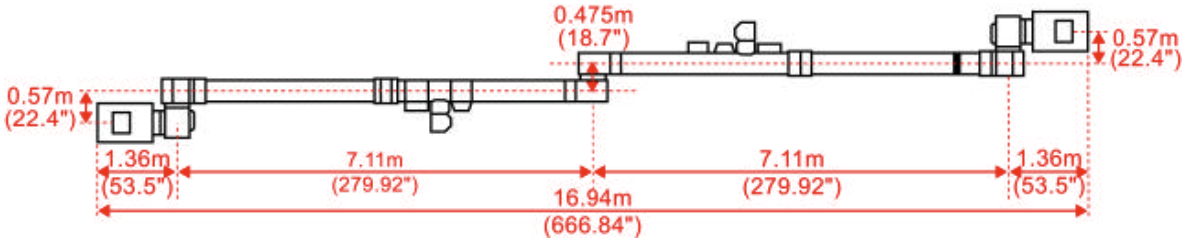
\includegraphics[scale=0.3]{SSRMS_dimensions.png}
  \caption{SSRMS Dimensions [4].}
  \label{SSRMS_dim}
\end{figure}
\begin{figure}[b]
  \centering
  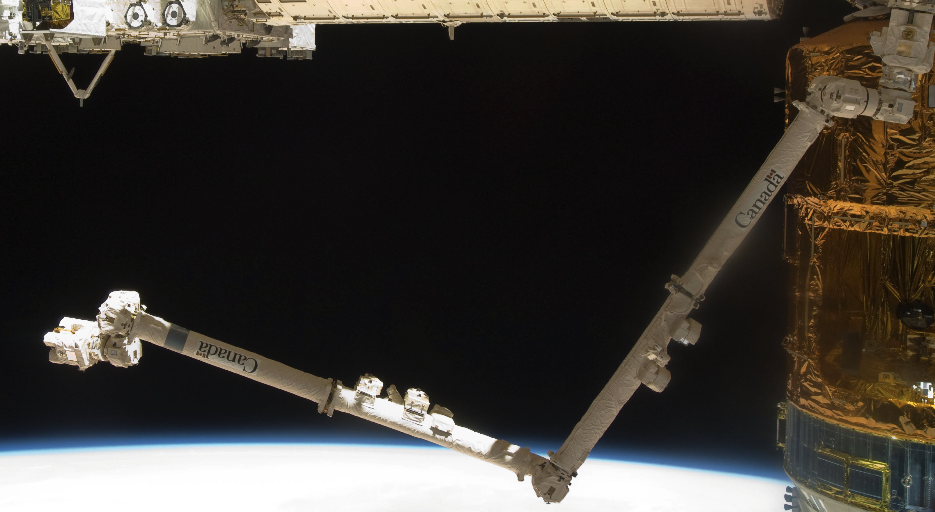
\includegraphics[scale=0.35]{SSRMS_orbit.png}
  \caption{The SSRMS on orbit [7].}
  \label{SSRMS_orbit}
\end{figure}
\newpage
\subsection{SPDM}
The SPD is a highly dexterous dual-armed robot, with two shoulders that provide support for the arms.\\
Each arm has seven joints, terminating with an Orbit Replacement Unit/Tool Changeout Mechanism (OTCM), the mechanism through which the SPDM arm interfaces with payloads and tools. The SPDM is also equipped with lights, video equipment, a tool platform and four tool holders.\\
The SPDM's primary role is to carry out delicate maintenance and servicing tasks on the International Space Station. Tasks include installing and removing small payloads such as batteries, power supplies and computers; operate robotic tools such as specialized wrenches and socket extensions; provide power and data connectivity to payloads; manipulate, install, remove and inspect scientific payloads.\\
It works near the Canadarm2 and can be grapped by it to be moved around.
\begin{figure}[h]
  \centering
  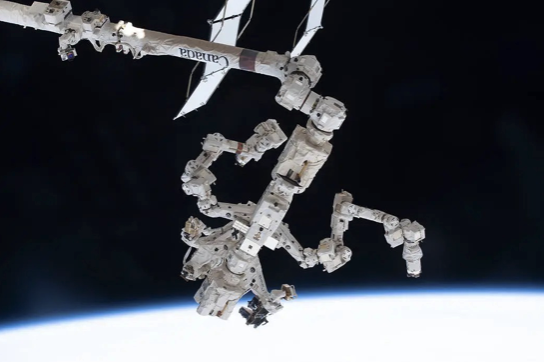
\includegraphics[scale=0.6]{SPDM.png}
  \caption{The SPDM on orbit.}
  \label{SPDM_orbit}
\end{figure}
\subsection{JEMRMS}
The JEMRMS system is used primarily for experiment payload handling. It consists of three major subsystems, the
Console, Main Arm (MA), and Small Fine Arm (SFA).\\
The Main Arm (MA) is a 10m, six-degree-of-freedom robot arm. It consists of three booms, six joints, an end effector on the tip, and two vision systems (one on the shoulder, the other on the tip).\\
The Small Fine Arm (SFA) is also asix-degree-of-freedom robot arm. It can perform more dexterous tasks than the MA. During operation, the SFA is grappled by the MA and receives power and data from the MA. The 2m SFA consists of two booms, six joints, and an end effector on the tip called the “tool,” and a camera on the tool. The tool has a force and torque sensor inside it for compliance operation [8].\\
\begin{figure}[h]
  \centering
  \subfloat[][\emph{Main Arm (MA).}]
  {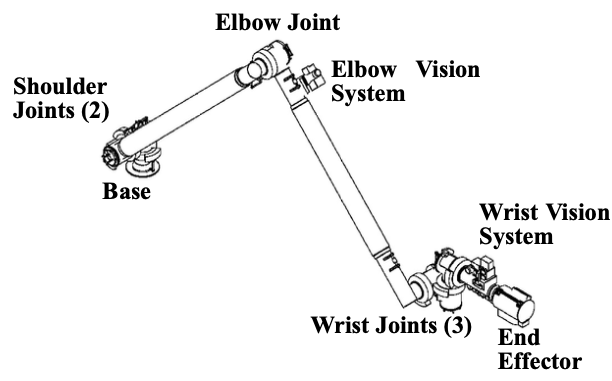
\includegraphics[scale=0.35]{MA.png}\label{unitary}} \quad
\subfloat[][\emph{Small Fine Arm (SFA).}]
  {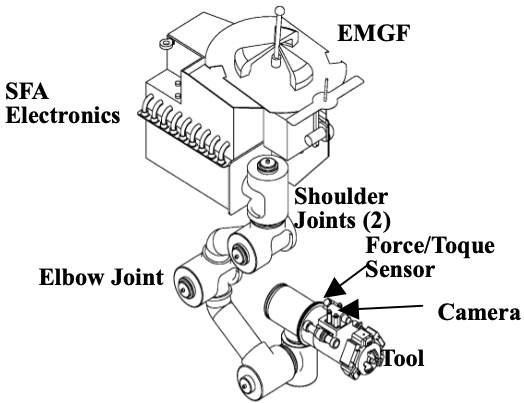
\includegraphics[scale=0.35]{SFA.png}\label{normal}} 
  \caption{The JEMRMS components. [8]}
  \label{JEMRMS_components}
\end{figure}
The JEM RMS end effector was designed based on the Shuttle RMS (SRMS) end effector. The grapple fixtures compatible with the JEMRMS MA can also be grappled by the SSRMS [4].
\newpage
\subsection{ERA}
The ERA is used on the Russian segment (RS) of the ISS. Specific tasks for the ERA include: installing, removing or replacing experiment payloads
and large Station elements; transferring small payloads in and out of the Station through the Russian airlock; transporting crew members from one external working site
to another; freeing cosmonauts to do other work during spacewalks; using its cameras to inspect the outside of the Space Station.
The ERA manipulator arm spans 11.3m and has 7 inline joints in a symmetric configuration with respect to the elbowjoint (Figure 2). It has a shoulder with 3 DOFs, an elbow with 1 DOF and a wrist with 3 DOFs. Both the shoulder andwrist contain three functionally identical joints with mutually perpendicular rotation axes.\\
The ERA has two end effectors (EE) which can act as a base, enabling either end of the ERA to be used as the shoulder. Thus the wrist and shoulder are operationally interchangeable, just as in the SSRMS design. The identical EE’s are able to grapple and ungrapple an ERA grapple fixture, transferring power or data to an external device/load. The EE also has an Integrated Service Tool (IST) which is a built-in motorized "screwdriver" that can provide mechanical torque
actuation.\\
The ERA is equipped with four Camera and Lighting Units (CLU) one on each EE and one on either side of the elbow. The CLU will be used to provide video images of operational tasks and, if necessary, to illuminate the scene and to act as an optical sensor to enable proximity control of a target during approach of a basepoint or grapple fixture in closed loop. The proximity control function enables ERA to approach grapple fixtures automatically and smoothly [4].
\begin{figure}[h]
  \centering
  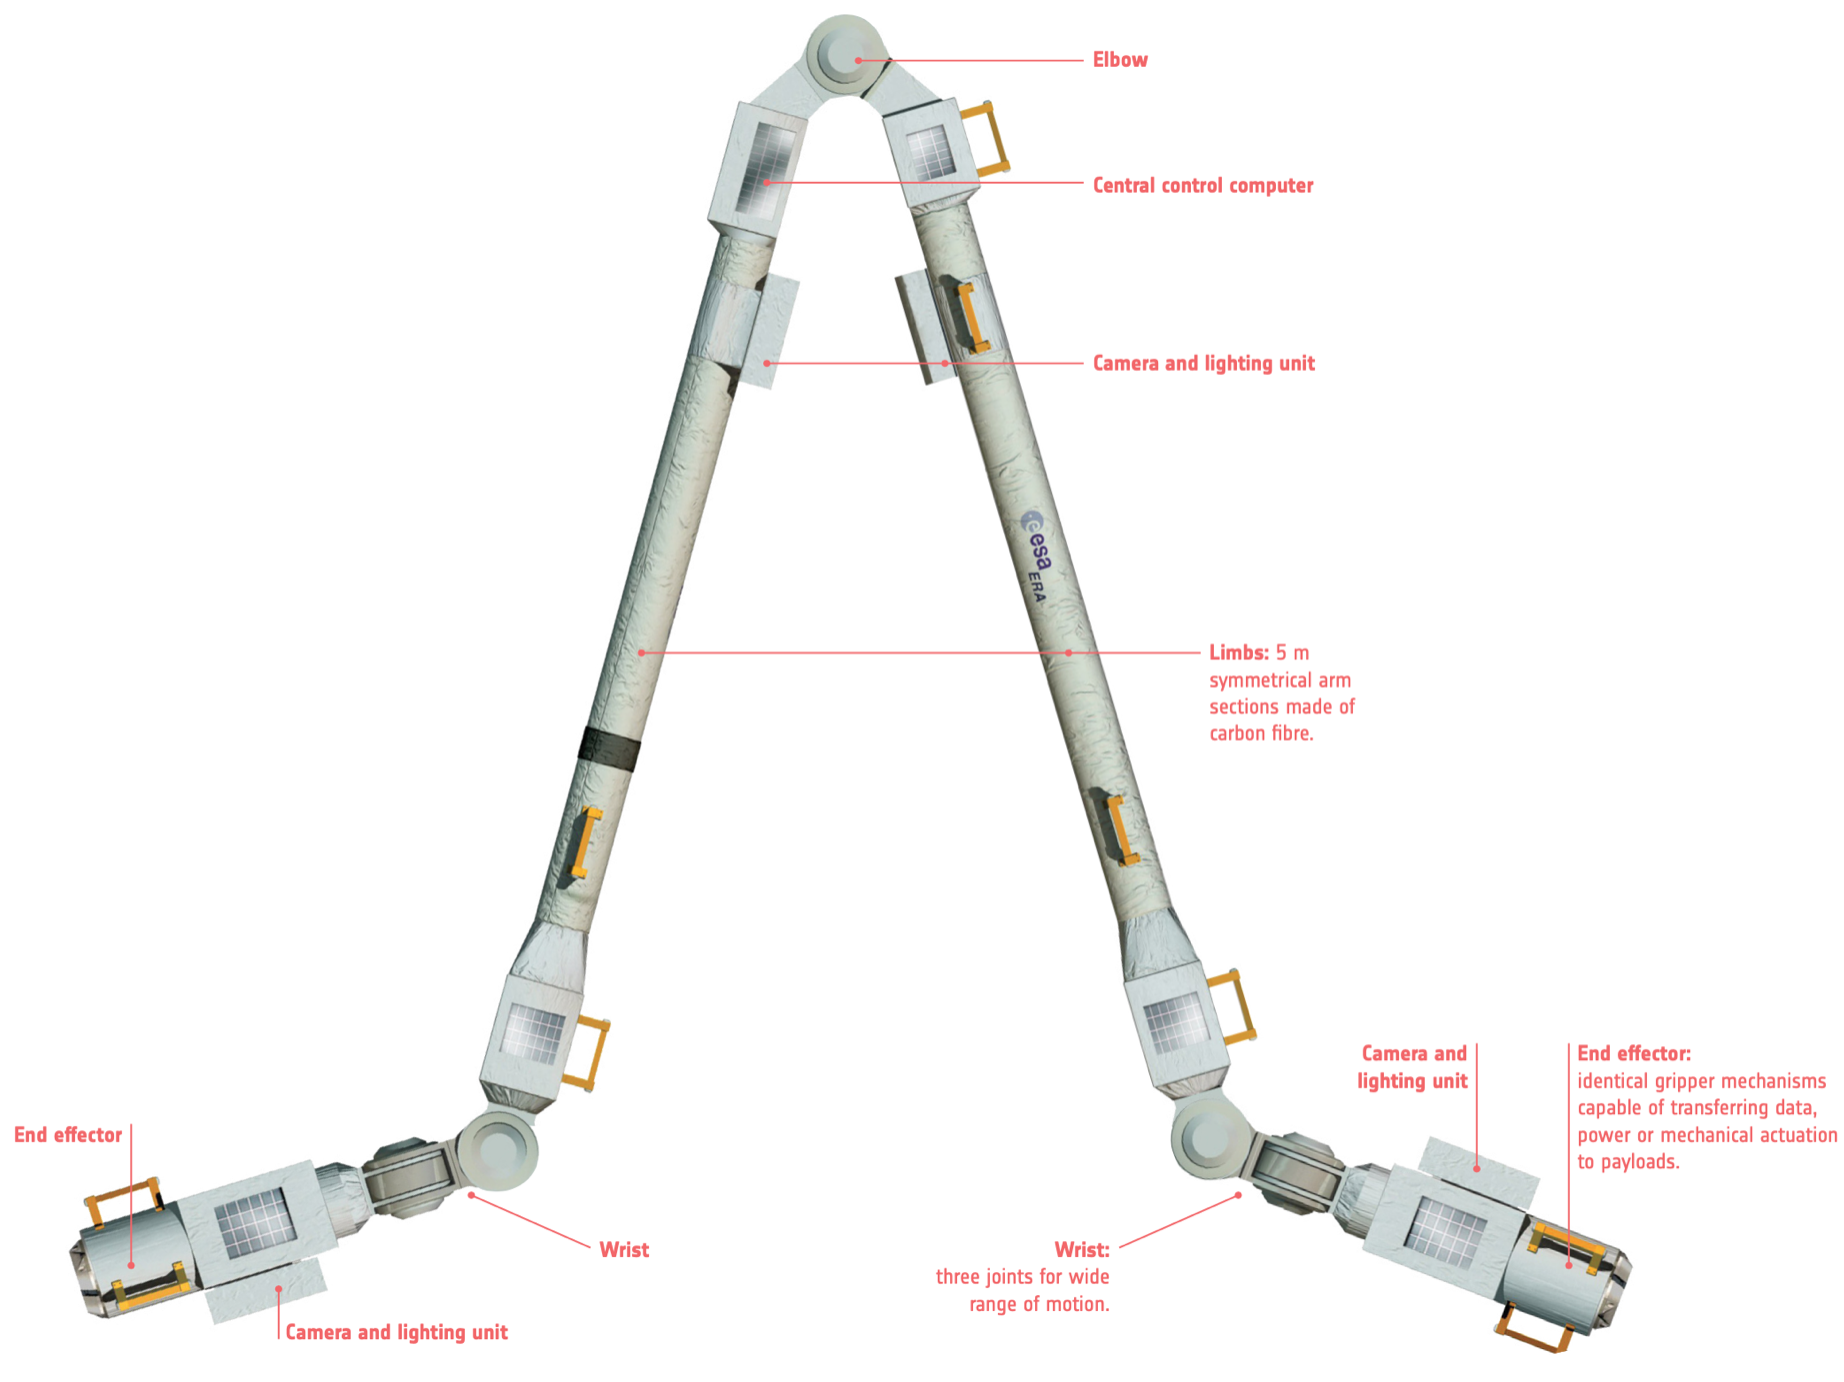
\includegraphics[scale=0.4]{ERA.png}
  \caption{ERA's components.} 
  \label{ERA}
\end{figure}
\subsection{RMSs Comparison}
To conlcude, The 7DOF design of the European and Canadian arms provide an extra degree of freedom that will enable both manipulators to access tight workspaces and avoid ISS structure during operations. This is particularly important when working in areas that have exposed station structure. The 7th DOF also allows for Arm Pitch Plane Change manoeuvres to avoid structure without changing the end effector position.\\
The maximum handling payloads the manipulators can capacity also dictates the type of grasp. The SSRMS is capable of handling payloads that have an equivalent mass to the Orbiter. The ERA is designed for slightly smaller payloads such as solar panels.\\
The ERA and the JEMRMS provide much finer position accuracy than the SSRMS: smaller payloads require more precise alignment. Also, the force moment sensor is always used for ERA and JEM operations and is optional for SSRMS operations. This FMS capability facilitates “peg in the hole” type of operations.
In the Table \ref{SRMs_comparison} the specifications of the SSRMS, ERA and JEMRMS are reported [4].
  \begin{table}[h]
    \caption{SSRMS, ERA and JEMRMS specifications [4].}
    \label{SRMs_comparison}
    \begin{center}
    \begin{tabular}{lccc}
      \toprule
    & \textbf{SSRMS} & \textbf{ERA} & \textbf{JEMRMS (MA)}\\
    \midrule
    Span&\SI{14.22}{\metre}&\SI{11.3}{\metre}&\SI{9.91}{\metre}\\
    Boom Span&\SI{7.11}{\metre}&\SI{7.77}{\metre}&\SI{3.93}{\metre}\\
    DOFs&7&7&6\\
    Joints&Offset&Inline&Offset\\
    Base&Relocatable&Relocatable&Fixed\\
    Positioning Accuracy&\SI{65}{\milli\metre}, \SI{0.71}{\degree}&\SI{40}{\milli\metre}, \SI{1}{\degree}&\SI{50}{\milli\metre}, \SI{1.8}{\degree}\\
    Mass&\SI{1336}{\kilogram}&\SI{630}{\kilogram}&\SI{757}{\kilogram}\\
    Max Handling Capacity&\SI{116}{\mega\gram}&\SI{8}{\mega\gram}&\SI{7}{\mega\gram}\\
    Power Consumption&\SI{1360}{\watt} (average)&>\SI{800}{\watt}&\SI{2.3}{\kilo\watt}\\
    \bottomrule
    \end{tabular}
    \end{center}
    \end{table}
\chapter{Kinematics}\label{kinematics}
What is a robot, then? In the previous chapter we have seen an overview of the actual reality of the space robotics field, but a proper definition of a what a robot is has not been given. A robot is a re-programmable machine for manipulation, positioning, orientation, machining of bodies able to interact with the environment, with a certain level of autonomy.\\
A robot is not just an automated machine, it is something more: takes decisions autonomously, can do different things at different times, is flexible.\\
According to [11] there are two main families of robots:
\begin{itemize}
  \item serial robots: a set of bodies rigidally connected by joints in an open kinematic chain.
  \item parallel robots: a set of bodies connected in a closed kinematic chain. They can withstand/produce a larger force.
\end{itemize}
A kinematic chain is therefore the concatenation of single degree of freedom (i.e. the minimum amount of indipendent coordinates that define the configuration of the robot) links. The joints can be revolute, prismatic or spherical, depending on the movement allowed by them (plane rotational, translational or 3D rotatonal respectively).\\
Grubler equation for palanar mechanisms gives the overall DoFs of a multibody system:
\begin{equation}
  n = 3(m-1)-2c_1-c_2
  \label{grubler}
\end{equation}
where $m$ is the number of rigid bodies attached to the base, $c_1$ and $c_2$ are class 1 and class 2 joints respectively, depending on how many DoFs do they allow (one or two). Revolute joints allows one DoF, i.e. rotation around their axes.\\
Whenever $n<n_j$, where $n_J$ is the number of joints, a redundancy occurs, meaning that the system has more joints than the dimension of the task space [11].\\
A very important definition for serial robots is the end defector (EE), i.e the point of the chain dedicated to the programmed task, as shown in Figure \ref{end_defector} in red.\\
Studying the kinematics of a mechanical system (such as a robot) refers to the calculation of the position and orientation of its end-effector frame from its joint coordinates [11].\\
\begin{figure}[!]
  \centering
  \begin{tikzpicture}

  % Definizione delle lunghezze dei bracci
  \def\lone{4} % Lunghezza del primo braccio
  \def\ltwo{3.5} % Lunghezza del secondo braccio

  % Angoli dei giunti
  \def\thetaone{30} % Angolo del primo giunto (in gradi)
  \def\thetatwo{45} % Angolo del secondo giunto (in gradi)

  % Coordinate del primo giunto
  \coordinate (O) at (0,0);

  % Calcolo delle coordinate del secondo giunto
  \coordinate (A) at ({\lone*cos(\thetaone)},{\lone*sin(\thetaone)});

  % Calcolo delle coordinate dell'end effector
  \coordinate (B) at ({\lone*cos(\thetaone) + \ltwo*cos(\thetaone + \thetatwo)}, 
                      {\lone*sin(\thetaone) + \ltwo*sin(\thetaone + \thetatwo)});

  % Disegno del primo braccio
  \draw[thick, black] (O) -- (A);

  % Disegno del secondo braccio
  \draw[thick, black] (A) -- (B);

  % Disegno assi
  \draw[thick,black,->] (0,0) -- (0,6) node[anchor=east]{y};
    \draw[thick,black,->] (0,0) -- (6,0) node[anchor=west]{x};

  % Rappresentazione dei giunti
  \filldraw[fill=black] (O) circle (0.1); % Base del manipolatore
  \filldraw[fill=black] (A) circle (0.1); % Primo giunto
  \filldraw[fill=red] (B) circle (0.1);   % End effector

  % Etichette
  \node[anchor=east] at (O) {$O$};
  \node[anchor=north] at (A) {$A$};
  \node[anchor=west] at (B) {$B$};

\end{tikzpicture}
  \caption{2D RR (revolute-revolute) manipulator.}
  \label{end_defector}
\end{figure}
We will now analyze the forward kinematics of a manipulator mounted on top of a mobile base, to form a vehicle-manipulator system (VMS) that can be controlled as a whole.\\
Starting from a simple model of the VMS, it will be possible to analyze its behaviour before and after the impact with an external object (i.e. meteorite or satellite).
\newpage
\section{Fundamental of Kinematics}\label{Homogeneous}
In this thesis, the kinematics chain have been evaluated by means of the "Homogeneous Matrix Approach" shown in [9,10]. For such approach, a briefly summary of notation is here presented.
\subsection{Roto-Translation Matrix}
Given two vectors in an $xy$ plane, only rotated without distortion, as in Figure~\ref{rotation_vectors}, the relationship between them can be found in the following way:
\begin{equation}
  v_2=\begin{bmatrix}
    v_{x_2}\\
    v_{y_2}
  \end{bmatrix}=\begin{bmatrix}
    v_{x_1}\cos{\theta}-v_{y_1}\sin{\theta}\\
    v_{x_1}\sin{\theta}+v_{y_1}\cos{\theta}
  \end{bmatrix}=\begin{bmatrix}
    \cos{\theta} & -\sin{\theta}\\
    \sin{\theta} & \cos{\theta}
  \end{bmatrix}\begin{bmatrix}
    v_{x_1}\\
    v_{y_1}
  \end{bmatrix}=R(\theta)v_1
  \label{rotation_matrix}
\end{equation}
\begin{figure}[h]
  \centering
  \begin{tikzpicture}

  \def\alpha{25}
  \coordinate (O) at (0,0);
  \coordinate (v1) at (3,1);
  \coordinate (v10) at (0.7*3,0.7*1);
  \coordinate (v11) at (0.7*3,0.7*1+0.3);
  \coordinate (v2) at ({3*cos(\alpha)-sin(\alpha)},{3*sin(\alpha)+cos(\alpha)});

  \draw[thick, black,->] (O) -> (v1);
  \draw[thick, red,->] (O) -> (v2);
  % \draw[thick, ->] (v1) arc (v2);

  % \draw (v1) arc(0:\theta:2 and 2) (v2);
  \draw[thick,->] (v10) arc [start angle=0, end angle=\alpha, x radius=2.4, y radius=2.4];


  \draw[thick,black,->] (0,0) -- (0,6) node[anchor=east]{$y$};
  \draw[thick,black,->] (0,0) -- (6,0) node[anchor=west]{$x$};


  \node[anchor=west] at (v1) {$v_1$};
  \node[anchor=south] at (v2) {$v_2$};
  \node[anchor=south west] at (v11) {$\theta$};

\end{tikzpicture}
  \caption{Vecors $v_2$ is rotate by $\theta$ withh respect to $v_1$.}
  \label{rotation_vectors}
\end{figure}
where $R_{\theta}$ is the rotation matrix.\\
We can use the same matrix to describe another transformation, i.e. to find the coordinated of a point initially defined with respect to a mobile frame, with respect to another frame, such as a fixed one (Figure~\ref{rotation_point}):
\begin{equation}
  \prescript{f}{}{P}=\prescript{f}{m}{R(\theta)}\prescript{m}{}{P}
\end{equation}
\begin{figure}[h]
  \centering
  \begin{tikzpicture}
  
  \coordinate (O) at (0,0);
  \coordinate (P) at (3,2);
  \coordinate (x0) at (6,0);
  \coordinate (x01) at ({0.7*6},0);
  \coordinate (x02) at ({0.7*6},0.5);
  \coordinate (y0) at (0,6);

  \def\alpha{15}

  \draw[thick, black] (O) -- (P);

  \draw[thick,black,->] (0,0) -- (y0) node[anchor=east]{$y_f$};
  \draw[thick,black,->] (0,0) -- (x0) node[anchor=west]{$x_f$};
  \filldraw[fill=black] (P) circle (0.1);

  \draw[thick,red,->] (0,0) -- ({-6*sin(\alpha)},{6*cos(\alpha)}) node[anchor=east]{$y_m$};
  \draw[thick,red,->] (0,0) -- ({6*cos(\alpha)},{6*sin(\alpha)}) node[anchor=west]{$x_m$};

  \draw[thick,->] (x01) arc [start angle=0, end angle=\alpha, x radius=4, y radius=4];

  \node[anchor=west] at (x02) {$\theta$};
  \node[anchor=west] at (P) {$P$};

\end{tikzpicture}
  \caption{The same point can be described with respect to both a fixed and a rotated mobile frame (in red).}
  \label{rotation_point}
\end{figure}
The notation used here is the following: the left superscript indicates the reference frame in which the point or the vector is referred to: $\prescript{m}{}{P}$ referes to the point $P$ with coordinate written with respect to the mobile frame. The matrix $\prescript{f}{m}{R(\theta)}$ "translates" a point described in the mobile frame to the fixed frame.\\
An important property of the rotation matrix is that it is orthogonal, hence its inverse is equal to its transpose.\\
We can concatenate the rotational matrices such that we can describe a point in a given reference frame to another one if we know all the relative rotational matrices of the frames between the two we are interested in:
\begin{equation}
  \prescript{0}{}{P}=\prescript{0}{1}{R(\theta)}\prescript{1}{2}{R(\theta)}\prescript{2}{}{P}
  \label{concatenate}
\end{equation}
This concept can be expanded easily in the 3D case, noticing that the columns of $R(\theta)$ in (\ref{rotation_matrix}) are the unit vectors of the moving (new) frame written in the fixed (old) frame. In this way, rotation matrices along the x, y and z axis are found [6]:
\begin{equation}
  \begin{array}{c}
  R_x(\phi)=\begin{bmatrix}
    1&0&0\\
    0&\cos{\phi}&-\sin{\phi}\\
    0&\sin{\phi}&\cos{\phi}
  \end{bmatrix} \quad R_y(\psi)=\begin{bmatrix}
    \cos{\psi}&0&\sin{\psi}\\
    0&1&0\\
    -\sin{\psi}&0&\cos{\psi}
  \end{bmatrix} \\
  R_z(\theta)=\begin{bmatrix}
    \cos{\theta}&-\sin{\theta}&0\\
    \sin{\theta}&\cos{\theta}&0\\
    0&0&1
  \end{bmatrix} 
\end{array}
\label{rotation_matrices}
\end{equation}
When a translation occurs, as shown in Figure~\ref{translation}, the transformation becomes:
\begin{equation}
  \prescript{f}{}{\{O_fP\}}=\prescript{f}{}{\{O_fO_m\}}+\prescript{f}{}{\{O_mP\}}=\prescript{f}{}{\{O_fO_m\}}+\prescript{m}{f}{R}\prescript{m}{}{\{O_mP\}}
\end{equation}
which can be written as follows:
\begin{equation}
  \prescript{f}{}{\begin{bmatrix}
    O_fP_x\\
    O_fP_y\\
    O_fP_z\\
    1
  \end{bmatrix}}=\begin{bmatrix}
    \prescript{f}{m}{R}&\prescript{f}{}{\begin{bmatrix}
      O_fO_mx\\
      O_fO_my\\
      O_fO_mz\\
    \end{bmatrix}}\\
    \mathbf{0}&1
  \end{bmatrix}\prescript{m}{}{\begin{bmatrix}
      O_mP_x\\
      O_mP_y\\
      O_mP_z\\
      1
    \end{bmatrix}}=\prescript{f}{m}{M}\prescript{m}{}{\begin{bmatrix}
      O_mP_x\\
      O_mP_y\\
      O_mP_z\\
      1
    \end{bmatrix}}
\label{roto_translation}
\end{equation}
where $\mathbf{0} \in \mathbb{R}^{3\times1}$ and $\prescript{m}{f}{M} \in \mathbb{R}^{4\times4}$ is called the \textit{Roto-Translational Matrix} or \textit{Homogeneous Transformation Matrix}, for which the same properties seen in equation~(\ref{concatenate}) hold. A fourth component has been appended at the end of the vectors, which is 1, since the Homogeneous Matrix would have had three rows but four columns otherwise. In this way it is squared and invertible, and $\prescript{0}{1}{M}^{-1}=\prescript{1}{0}{M}$.
\begin{figure}[h]
  \centering
  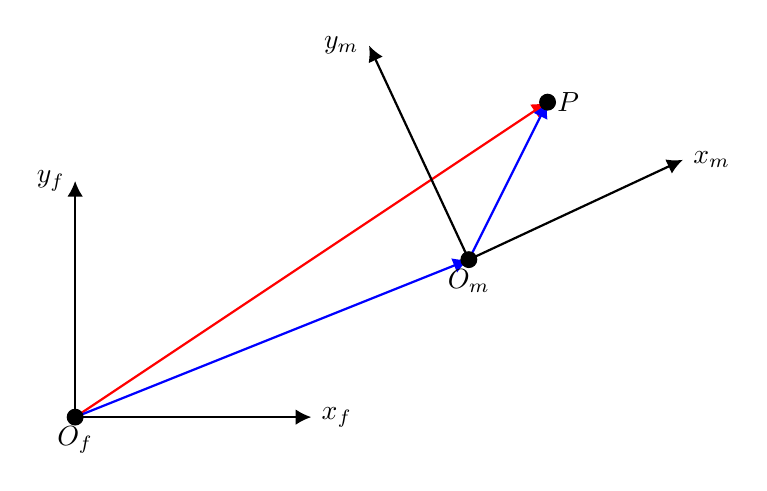
\begin{tikzpicture}

  \def\alpha{25}

  \coordinate (Of) at (0,0);
  \coordinate (Om) at (5,2);
  \coordinate (P) at (6,4);
  \coordinate (xf) at (3,0);
  \coordinate (yf) at (0,3);
  \coordinate (xm) at ({5+3*cos(\alpha)},{2+3*sin(\alpha)});
  \coordinate (ym) at ({5-3*sin(\alpha)},{2+3*cos(\alpha)});

  \draw[thick, red,->,] (Of) -- (P);
  \draw[thick, blue,->] (Of) -- (Om);
  \draw[thick, blue,->] (Om) -- (P);

  \draw[thick,black,->] (Of) -- (yf) node[anchor=east]{$y_f$};
  \draw[thick,black,->] (Of) -- (xf) node[anchor=west]{$x_f$};
  \filldraw[fill=black] (P) circle (0.1);
  \filldraw[fill=black] (Om) circle (0.1);
  \filldraw[fill=black] (Of) circle (0.1);

  \draw[thick,black,->] (Om) -- (ym) node[anchor=east]{$y_m$};
  \draw[thick,black,->] (Om) -- (xm) node[anchor=west]{$x_m$};

  \node[anchor=west] at (P) {$P$};
  \node[anchor=north] at (Om) {$O_m$};
  \node[anchor=north] at (Of) {$O_f$};

\end{tikzpicture}
  \caption{Definition of a point in a rotated and translated frame with respect to the fixed one. The position of $P$ with respect to the fixed frame (red arrow) can be seen as the sum of the position of the moving frame $O_m$ with respect of $O_f$ and the relative position of $P$ in the moving frame, both in blue.}
  \label{translation}
\end{figure}
\newpage
\subsection{Velocity Matrix}\label{velocity_section}
Given the same point in Figure~\ref{translation} is is possible to find the velocity of the point with respect to the fixed frame. By derivation of equation (\ref{roto_translation}) one can get:
\begin{equation}
  \prescript{f}{}{\{\dot{O_fP}\}}=\prescript{f}{m}{\dot{M}}\prescript{m}{}{\{O_mP\}}+\prescript{f}{m}{M}\prescript{m}{}{\{\dot{O_mP}\}}
\end{equation}
and since $\prescript{m}{}{\{\dot{O_mP}\}}=0$, assuming the point fixed in the mobile frame, and $\prescript{m}{}{\{O_mP\}}=\prescript{m}{f}{M}\prescript{f}{}{\{O_fP\}}$:
\begin{equation}
  \prescript{f}{}{\{\dot{O_fP}\}}=\prescript{f}{m}{\dot{M}}\prescript{m}{f}{M}\prescript{f}{}{\{O_fP\}}=\prescript{f}{}{W}\prescript{f}{}{\{O_fP\}}
  \label{velocity_matrix}
\end{equation}
with $\prescript{f}{}{W}$ the \textit{Velocity Matrix}.\\
The Velocity Matrix can be generalized as follows [9]:
\begin{equation}
  W=\begin{bmatrix}
    0&-\omega_z&\omega_y&v_x\\
    \omega_z&0&-\omega_x&v_y\\
    -\omega_y&\omega_x&0&v_z\\
    0&0&0&0
  \end{bmatrix}
\end{equation}
where $\omega$ indicates the angular velocity of the body and $v$ is the velocity of the point, considered belonging to the body that in a considered instant is passing through the origin of the reference frame.\\
The composition of the Velocity Matrix follows the Rival's Theorem (see Figure~\ref{rival}):
\begin{equation}
  \prescript{n}{}{W_{02}}=\prescript{n}{}{W_{01}}+\prescript{n}{}{W_{12}}
  \label{composition}
\end{equation}
\begin{figure}[h]
  \centering
  \begin{tikzpicture}

  \def\alpha{25}
  \def\beta{-15}

  \coordinate (O1) at (0,0);
  \coordinate (O2) at (5,2);
  \coordinate (O3) at (8,-1);
  \coordinate (P) at (10,0);
  \coordinate (x1) at (3,0);
  \coordinate (y1) at (0,3);
  \coordinate (x2) at ({5+3*cos(\alpha)},{2+3*sin(\alpha)});
  \coordinate (y2) at ({5-3*sin(\alpha)},{2+3*cos(\alpha)});
  \coordinate (x3) at ({8+3*cos(\beta)},{-1+3*sin(\beta)});
  \coordinate (y3) at ({8-3*sin(\beta)},{-1+3*cos(\beta)});

  \coordinate (d1) at (1,2);
  \coordinate (d2) at (7,4);
  \coordinate (d3) at (1.5,-1.5);

  \draw[thick,black,->] (O1) -- (y1) node[anchor=east]{$y_0$};
  \draw[thick,black,->] (O1) -- (x1) node[anchor=west]{$x_0$};

  \draw[thick,black,->] (O2) -- (y2) node[anchor=east]{$y_1$};
  \draw[thick,black,->] (O2) -- (x2) node[anchor=west]{$x_1$};

  \draw[thick,black,->] (O3) -- (y3) node[anchor=east]{$y_2$};
  \draw[thick,black,->] (O3) -- (x3) node[anchor=west]{$x_2$};

  \def\myshift#1{\raisebox{2ex}}
  \draw[red,->,thick,postaction={decorate,decoration={text along path,text align=center,text={|\myshift|W01}}}] (d1) arc[start angle=130,end angle=90,radius=4cm];
  \draw[red,->,thick,postaction={decorate,decoration={text along path,text align=center,text={|\myshift|W12}}}] (d2) arc[start angle=130,end angle=-10, x radius=2, y radius=1.5];
  \draw[red,->,thick,postaction={decorate,decoration={text along path,text align=center,text={|\myshift|W02}}}] (d3) arc[start angle=-180,end angle=-20, x radius=3.5, y radius=2];

  \filldraw[fill=black] (P) circle (0.1);
  \filldraw[fill=black] (O2) circle (0.1);
  \filldraw[fill=black] (O1) circle (0.1);
  \filldraw[fill=black] (O3) circle (0.1);

  \node[anchor=west] at (P) {$P$};
  \node[anchor=north] at (O2) {$O_1$};
  \node[anchor=north] at (O1) {$O_0$};
  \node[anchor=north] at (O3) {$O_2$};

\end{tikzpicture}
  \caption{Rival's Theorem for velocities composition. The three transformation $W_{01}$, $W_{12}$ and $W_{02}$ are also called \textit{Drag Motion}, \textit{Relative Motion} and \textit{Absolute Motion} respectively.}
  \label{rival}
\end{figure}
which is true only when all the matrices are projected in the same frame $n$.\\
The notation used in equation (\ref{composition}) has to be read in the following way: $\prescript{n}{}{W}_{02}$ is the Velocity Matrix of frame two with respect to frame zero, projected in frame $n$.\\
Is is also possible to change the frame in which the matrix is projected:
\begin{equation}
  \prescript{m}{}{W}=\prescript{m}{n}{M}\prescript{n}{}{W}\prescript{n}{m}{M}
  \label{change_frame}
\end{equation}

Some attention must be given also to the matrix representing a "boolean" interpretation of the rotation: the $L$ matrix. For the aim of this thesis, and as it is introduced in [10], this matrix can be easily obtained from its Velocity Matrix dividing it by the module of its angular (or linear, when there is translation) velocity:
\begin{equation}
  L=\frac{W}{|\omega|}
  \label{L_matrix}
\end{equation}
where $|\omega|=\sqrt{\omega_x^2+\omega_y^2+\omega_z^2}$.\\
Given the robotic focus of this work, these calculations will be quite straightforward once defined the axis of rotation of a link. For a revolute joint, for example, the Velocity Matrix with respect of the joint frame will be:
\begin{equation}
  W=\begin{bmatrix}
    0&-\dot{\alpha}&0&0\\
    \dot{\alpha}&0&0&0\\
    0&0&0&0\\
    0&0&0&0
  \end{bmatrix}
\end{equation}
with $\dot{\alpha}=\omega_z$, and the "logic" of the rotation is thus given by $L$:
\begin{equation}
  L=\frac{W}{\dot{\alpha}}=\begin{bmatrix}
    0&1&0&0\\
    1&0&0&0\\
    0&0&0&0\\
    0&0&0&0
  \end{bmatrix}
  \label{L_matrix}
\end{equation}
\newpage
\subsection{Danavit-Hartenberg Method}
To define the reference frames fixed to the links of a serial manipulator, one can follow the Danavit-Hartenberg algorithm, which guarantees a coherent and functional mehod through all the calculations. It has been thought for robots with revolute joints.\\
It follows this ordered procedures:
\begin{enumerate}
  \item $z_i$ axis: axis of the revolute joint which connects the link to the following.
  \item $x_i$ axis: line of minimum distance between $z_{i-1}$ and $z_i$, oriented from $z_{i-1}$ to $z_i$.
  \item $y_i$ axis: obtained by the vectorial product of the other two axes.
\end{enumerate}
In Figure~\ref{DH}, a DH convention for a planar serial manipulator has been used for configuration shown in Figure~\ref{end_defector}.
\begin{figure}[h]
  \centering
  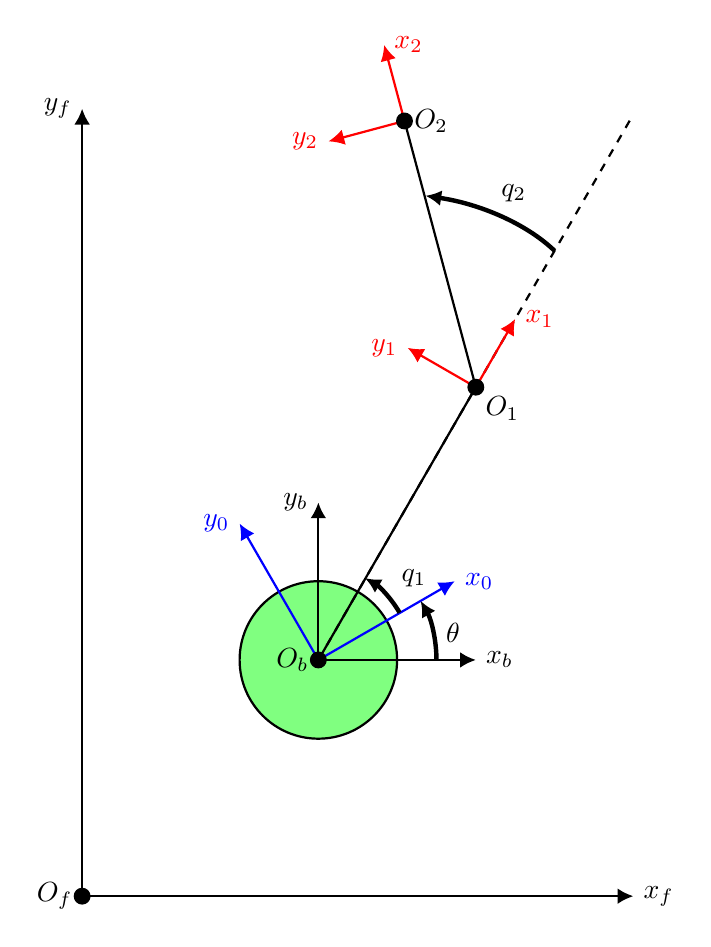
\begin{tikzpicture}

  \def\lone{4} 
  \def\ltwo{3.5}

  \def\thetazero{30}
  \def\thetaone{30}
  \def\thetatwo{45} 

  \coordinate (O) at (0,0);
  \coordinate (Ob) at (3,3);
  \coordinate (Ob0) at ({-0.7+3+2*cos(\thetazero)},{-0.4+3+2*sin(\thetazero)});
  \coordinate (Ob01) at ({-0.8+3+2*cos(\thetazero)},{-0.2+3+2*sin(\thetazero)});
  \coordinate (A) at ({3+\lone*cos(\thetaone+\thetazero)},{3+\lone*sin(\thetaone+\thetazero)});
  \coordinate (C) at ({3+2*\lone*cos(\thetaone+\thetazero)},{3+2*\lone*sin(\thetaone+\thetazero)});
  \coordinate (C0) at ({3+1.5*\lone*cos(\thetaone+\thetazero)},{3+1.5*\lone*sin(\thetaone+\thetazero)});
  \coordinate (C01) at ({3-0.8+1.5*\lone*cos(\thetaone+\thetazero)},{3+0.5+1.5*\lone*sin(\thetaone+\thetazero)});
  \coordinate (B) at ({3+\lone*cos(\thetaone+\thetazero) + \ltwo*cos(\thetaone + \thetatwo+\thetazero)}, 
                      {3+\lone*sin(\thetaone+\thetazero) + \ltwo*sin(\thetaone + \thetatwo+\thetazero)});
  \coordinate (B0) at ({3+1.5*\lone*cos(\thetaone+\thetazero) + 1.5*\ltwo*cos(\thetaone + \thetatwo+\thetazero)}, 
                      {3+1.5*\lone*sin(\thetaone+\thetazero) + 1.5*\ltwo*sin(\thetaone + \thetatwo+\thetazero)});

  \draw[thick,fill=green!50] (3,3) circle (1);

  \draw[thick, black] (Ob) -- (A);
  \draw[thick, black, dashed] (Ob) -- (C);
  \draw[thick, black] (A) -- (B);

  \draw[thick,black,->] (O) -- (0,10) node[anchor=east]{$y_f$};
  \draw[thick,black,->] (O) -- (7,0) node[anchor=west]{$x_f$};

  \draw[thick,black,->] (Ob) -- (3,5) node[anchor=east]{$y_b$};
  \draw[thick,black,->] (Ob) -- (5,3) node[anchor=west]{$x_b$};

  \draw[thick,blue,->] (Ob) -- ({3-2*sin(\thetazero)},{3+2*cos(\thetazero)}) node[anchor=east]{$y_0$};
  \draw[thick,blue,->] (Ob) -- ({3+2*cos(\thetazero)},{3+2*sin(\thetazero)}) node[anchor=west]{$x_0$};
  

  \draw[thick,red,->] (A) -- ({3+\lone*cos(\thetaone+\thetazero)-sin(\thetaone+\thetazero)},{3+\lone*sin(\thetaone+\thetazero)+cos(\thetaone+\thetazero)}) node[anchor=east]{$y_1$};
  \draw[thick,red,->] (A) -- ({3+\lone*cos(\thetaone+\thetazero)+cos(\thetaone+\thetazero)},{3+\lone*sin(\thetaone+\thetazero)+sin(\thetaone+\thetazero)}) node[anchor=west]{$x_1$};

  \draw[thick,red,->] (B) -- ({3+\lone*cos(\thetaone+\thetazero)+ \ltwo*cos(\thetaone + \thetatwo+\thetazero)-sin(\thetaone+ \thetatwo+\thetazero)},{3+\lone*sin(\thetaone+\thetazero)+ \ltwo*sin(\thetaone + \thetatwo+\thetazero)+cos(\thetaone+ \thetatwo+\thetazero)}) node[anchor=east]{$y_2$};
  \draw[thick,red,->] (B) -- ({3+\lone*cos(\thetaone+\thetazero)+ \ltwo*cos(\thetaone + \thetatwo+\thetazero)+cos(\thetaone+ \thetatwo+\thetazero)},{3+\lone*sin(\thetaone+\thetazero)+ \ltwo*sin(\thetaone + \thetatwo+\thetazero)+sin(\thetaone+ \thetatwo+\thetazero)}) node[anchor=west]{$x_2$};

  \draw[ultra thick,->] (4.5,3) arc [start angle=0, end angle=\thetaone, x radius=1.5, y radius=1.5];
  \draw[ultra thick,->] (Ob0) arc [start angle=\thetazero, end angle={\thetaone+\thetazero}, x radius=1.2, y radius=1.2];
  \draw[ultra thick,->] (C0) arc [start angle=\thetaone, end angle={\thetatwo+\thetaone}, x radius=2.7, y radius=1.5];

  \filldraw[fill=black] (O) circle (0.1);
  \filldraw[fill=black] (Ob) circle (0.1);
  \filldraw[fill=black] (A) circle (0.1);
  \filldraw[fill=black] (B) circle (0.1);

  \node[anchor=east] at (O) {$O_f$};
  \node[anchor=east] at (Ob) {$O_b$};
  \node[anchor=north west] at (A) {$O_1$};
  \node[anchor=west] at (B) {$O_2$};
  \node[anchor=south west] at (4.5,3.1) {$\theta$};
  \node[anchor=south west] at (Ob01) {$q_1$};
  \node[anchor=south west] at (C01) {$q_2$};

\end{tikzpicture}
  \caption{The Danavit-Hartenberg rule has been used to place the local joints' frame (in red) in a planar RR manipulator, with arms length $l_1$ and $l_2$, mounted on top of a disk-shaped base (in green). The rotated frame of the base of the angle $\theta_o$ has been plotted in blue. Following the hand rule, the z axis is orthogonal to the plane.}
  \label{DH}
\end{figure}
\subsection{Jacobian Matrix}
Another important matrix in the analysis if a manipulator is the so called \textit{Jacobian Matrix}.\\
To study the direct kinematics of a manipulator, as already said, means to find the relationship between the end-defector position and orientation and its joints. When writing the position of the EE (denoted by S), we obtain a function of the robot's joints:
\begin{equation}
  S=f(q_1,q_2,\dots,q_n)
  \label{EE_position}
\end{equation}
where $q_i$ are the manipulators DoFs.\\
By derivation of (\ref{EE_position}) one can obtain:
\begin{equation}
  \dot{S}=J_a\dot{Q}
  \label{task_dimension}
\end{equation}
where $J_a$ is the \textit{Analytical Jacobian Matrix} and $Q=\{q_1,q_2,\dots,q_n\}$.\\
Its dimension are very important, since kinematic singularities, which are configurations in which the end-effector frame loses the ability to move or rotate in one or more directions, correspond to those configurations at which the Jacobian matrix fails to have maximal rank [11], where the rank is defined as the number of indipendent rows or couloumn of the matrix.\\
Singularities happen if the open-chain robot is kinematically redundant, meaning, as already mentioned, that it has more joints than the dimension of the task space; then the inverse of the jacobian doesn't exist anymore, since the inversion requires a squared full rank matrix. When this occurs, the pseudoinverse or \textit{Moore-Penrose Inverse} matrix, denoted by $J^+$, must be used:
\begin{equation}
  \begin{cases}
    J^+=(J^TJ)^{-1}J^T \quad \text{when J has linearly indipendent comlumns}\\
    J^+=J^T(JJ^T)^{-1} \quad \text{when J has linearly indipendent rows}
  \end{cases}
  \label{pseudoinverse}
\end{equation}
In robotics, the most common case is the one with a Jacobian with linearly indipendent columns, since it's common to have more links than dimensions in the task space.
\newpage
\section{Planar Vehicle-Manipulator System}\label{planar_VMS}
It will be now presented a simple case of Vehicle-Manipulator System, consisting in a base approximated with a disk and a planar serial manipulator whose revolute joints move around their z axis, orthoginal to the plane (as the one shown in Figure~\ref{DH}).\\
Since the aim of this work is to study the dynamics of the system after the catching of a tumbling object, its kinematics will be analyzed too, by considering it as a disk. The calculations will be shown as a reference for future more complex model, for which the matrices and joint positions will be omitted.\\
Firstly, let's define the DoFs of the VMS, which will be:
\begin{equation}
  p=\{x_b,y_b,\theta_b,q_1,q_2\}
\end{equation}
It is already clear that, being in the 2D case, the number of DoFs is greater than the dimension of the task space (i.e. $5>2$). In fact, from (\ref{grubler}), given $m=3$ (base and two arms) and $c_1=2$ (two revolute joints), we have $n=2$, while $p\in\mathbb{R} ^5$.\\ 
This means that a redundancy occurs and the pseudoinverse jacobian must be used instead of the inverse one, when needed.\\
The generalized coordinate of the tumbling object are the following:
\begin{equation}
  \psi=\{x_O,y_O,\theta_O\}
  \label{object_coordinates}
\end{equation}
Since the links rotate only aorund the local z-axis, given equations (\ref{rotation_matrices}) and (\ref{roto_translation}), the roto-translation matrices of the manipulator chain have the following form:
\begin{equation}
  \prescript{a}{f}{M}=
  \begin{bmatrix}
    \cos{\alpha}&-\sin{\alpha}&0&p_1\\
    \sin{\alpha}&\cos{\alpha}&0&p_2\\
    0&0&1&p_3\\
    0&0&0&1
  \end{bmatrix}
\end{equation}
where $p_1,p_2,p_3$ are the coordinates of the following moving frame in the chain projected in the actual frame.\\
Following the notation of Figure~\ref{DH}, the matrices are then given:
\begin{equation}
  \begin{array}{c}
    \prescript{f}{b}{M}=\begin{bmatrix}
      0&0&0&x_b\\
    0&0&0&y_b\\
    0&0&1&0\\
    0&0&0&1
    \end{bmatrix}\quad
    \prescript{b}{0}{M}=\begin{bmatrix}
      \cos{\theta_0}&-\sin{\theta_0}&0&0\\
      \sin{\theta_0}&\cos{\theta_0}&0&0\\
      0&0&1&0\\
      0&0&0&1
    \end{bmatrix}\\ \\
    \prescript{0}{1}{M}=\begin{bmatrix}
      \cos{q_1}&-\sin{q_1}&0&l_1\cos{q_1}\\
      \sin{q_1}&\cos{q_1}&0&l_1\sin{q_1}\\
      0&0&1&0\\
      0&0&0&1
    \end{bmatrix}\quad
    \prescript{1}{2}{M}=\begin{bmatrix}
      \cos{q_2}&-\sin{q_2}&0&l_2\cos{q_2}\\
      \sin{q_2}&\cos{q_2}&0&l_2\sin{q_2}\\
      0&0&1&0\\
      0&0&0&1
    \end{bmatrix}
  \end{array}
\end{equation}
with $l_1$ and $l_2$ the lenghts of the two arms.\\
The origin of the frames written in the fixed one can be found by multiplying the Homogeneous Matrix by $O_3=\{0,0,0,1\}$. Thus, the end-defector position is:
\begin{equation}
  p_{EE}=\prescript{0}{2}{M}O_3= \begin{bmatrix}
    l_1\cos{(\theta_0+q_1)}+l_2\cos{(\theta_0+q_1+q_2)}+x_b\\
    l_1\sin{(\theta_0+q_1)}+l_2\sin{(\theta_0+q_1+q_2)}+y_b\\0\\1
   \end{bmatrix}
   \label{EE_position}
\end{equation}
with $\prescript{0}{3}{M}=\prescript{f}{b}{M}\prescript{b}{0}{M}\prescript{0}{1}{M}\prescript{1}{2}{M}$ for the chain rule (\ref{concatenate}).\\
The Jacobian Matrix is then obtained by deriviation of $p_{EE}$ with respect to the VMS DoFs $p$ such that $\dot{p}_{EE}=J\dot{p}$:

\begin{equation}
  \begin{tiny}
  J=\begin{bmatrix}
    1&0&-l_1\sin{(\theta_0+q_1)}-l_2\sin{(\theta_0+q_1+q_2)}&-l_1\sin{(\theta_0+q_1)}-l_2\sin{(\theta_0+q_1+q_2)}&-l_2\sin{(\theta_0+q_1+q_2)}\\
    0&1&l_1\cos{(\theta_0+q_1)}+l_2\cos{(\theta_0+q_1+q_2)}&l_1\cos{(\theta_0+q_1)}+l_2\cos{(\theta_0+q_1+q_2)}&l_2\cos{(\theta_0+q_1+q_2)}
  \end{bmatrix}
\end{tiny}
\end{equation}
As already forecasted, the Jacobian Matrix is rectangular, i.e. $J\in \mathbb{R}^{2\times5}$, thus not invertibile.\\

Following equation (\ref{velocity_matrix}), the Velocity Matrices can be found as $\prescript{f}{}{W}=\prescript{f}{m}{\dot{M}}\prescript{m}{f}{M}$:
\begin{equation}
  \begin{array}{c}
    \prescript{f}{}{W_{fb}}=\prescript{f}{b}{\dot{M}}\prescript{b}{f}{M}=\begin{bmatrix}
      0&0&0&\dot{x_b}\\
      0&0&0&\dot{y_b}\\
      0&0&0&0\\
      0&0&0&0
    \end{bmatrix} \quad
    \prescript{b}{}{W_{b0}}=\prescript{b}{0}{\dot{M}}\prescript{0}{b}{M}=\begin{bmatrix}
      0&-\theta_0&0&0\\
      \theta_0&0&0&0\\
      0&0&0&0\\
      0&0&0&0
    \end{bmatrix}\\ \\
    \prescript{1}{}{W_{01}}=\begin{bmatrix}
      0&-q_1&0&0\\
      q_1&0&0&0\\
      0&0&0&0\\
      0&0&0&0
    \end{bmatrix} \quad
    \prescript{2}{}{W_{12}}=\begin{bmatrix}
      0&-q_2&0&0\\
      q_2&0&0&0\\
      0&0&0&0\\
      0&0&0&0
    \end{bmatrix}
  \end{array}
\end{equation}
where the notation is the same of equation (\ref{composition}).\\
Since it is of our interest (see Chapter \ref{dynamics}) to write all the velociti matrices projected in the fixed frame, following equation (\ref{change_frame}) it is possible to write:
\begin{equation}
    \prescript{f}{}{W_{b0}}=\prescript{f}{b}{M}\prescript{b}{}{W_{b0}}\prescript{b}{f}{M}=\begin{bmatrix}
      0&-\theta_0&0&y_b \dot{\theta_0}\\
      \theta_0&0&0&-x_b \dot{\theta_0}\\
      0&0&0&0\\
      0&0&0&0
    \end{bmatrix}
  \label{W_bo}
\end{equation}
Finally, now that both $\prescript{f}{}{W_{fb}}$ and $\prescript{f}{}{W_{b0}}$ are projected in the same frame, following equation (\ref{concatenate}):
\begin{equation}
    \prescript{f}{}{W_{f0}}=\prescript{f}{}{W_{fb}}+\prescript{f}{}{W_{b0}}=\begin{bmatrix}
      0&-\theta_0&0&\dot{x_b}+y_b \dot{\theta_0}\\
      \theta_0&0&0&\dot{y_b}-x_b \dot{\theta_0}\\
      0&0&0&0\\
      0&0&0&0
    \end{bmatrix}
    \label{arm_1_vel}
\end{equation}
and the same holds for $\prescript{f}{}{W_{f1}}$ and $\prescript{f}{}{W_{f2}}$, whose $3\times 3$ submatrices, related to the angular velocity, are:
  \begin{equation}
    \begin{array}{c}
      \prescript{f}{}{W_{{f1}_{1:3,1:3}}}=\begin{bmatrix}
        0&-\theta_0-q_1&0\\
        \theta_0+q_1&0&0\\
        0&0&0
      \end{bmatrix} \quad
      \prescript{f}{}{W_{{f1}_{1:3,1:3}}}=\begin{bmatrix}
        0&-\theta_0-q_1-q_2&0\\
        \theta_0+q_1+q_2&0&0\\
        0&0&0
      \end{bmatrix}
    \end{array}
    \label{arms_velocity}
  \end{equation}
\\
We could have calculated $\prescript{f}{}{W_{f0}}$ using equation (\ref{velocity_matrix}) as well ($\prescript{f}{}{W_{f0}}=\prescript{f}{0}{\dot{M}}\prescript{0}{f}{M}$). However, it is useful to have also the relative velocity matrices to calculate the corresponding $L$ matrices (see equation (\ref{L_matrix})):
\begin{equation}
  \begin{array}{c}
    \prescript{f}{}{L_{{fb}_x}}=\begin{bmatrix}
      0&0&0&1\\
      0&0&0&0\\
      0&0&0&0\\
      0&0&0&0
    \end{bmatrix} \quad
    \prescript{f}{}{L_{{fb}_y}}=\begin{bmatrix}
      0&0&0&0\\
      0&0&0&1\\
      0&0&0&0\\
      0&0&0&0
    \end{bmatrix}\\ \\
    \prescript{b}{}{L_{b0}}=\prescript{0}{}{L_{01}}=\prescript{1}{}{L_{12}}=\begin{bmatrix}
      0&-1&0&0\\
      1&0&0&0\\
      0&0&0&0\\
      0&0&0&0
    \end{bmatrix}
  \end{array}
  \label{L_matrices}
\end{equation}
where $\prescript{f}{}{L_{{fb}_x}}$ and $\prescript{f}{}{L_{{fb}_y}}$ have been found such that $\prescript{f}{}{L_{fb}}=\prescript{f}{}{L_{{fb}_x}}+\prescript{f}{}{L_{{fb}_y}}$.\\
By projecting in the fixed frame:
\begin{equation}
  \prescript{f}{}{L_{b0}}=\begin{bmatrix}
    0&-1&0&y_b\\
    1&0&0&-x_b\\
    0&0&0&0\\
    0&0&0&0
  \end{bmatrix}
\end{equation}
which is $\prescript{f}{}{W_{b0}}/ \dot{\theta}_0$ from equation (\ref{W_bo}).
\newpage
\subsection{Object's Kinematics}
For the planar case, the object to be captured (might it be a satellite or a micro-meteorite) is approximated with a  disk, in the same way we did for the base of the VMS.\\
The goal of the object's kinematics is to find the relationshipt between the velocity of its centre and the velocity of the contact point ($c_p$), as suggested in [12].\\
Hence, the Homogeneous Matrices related to the tumbling object are the following:
\begin{equation}
  \begin{array}{c}
    \prescript{f}{O_0}{M}=\begin{bmatrix}
      1&0&0&x_O\\
    0&1&0&y_O\\
    0&0&1&0\\
    0&0&0&1
    \end{bmatrix}\quad
    \prescript{O_0}{O_1}{M}=\begin{bmatrix}
      \cos{\theta_O}&-\sin{\theta_O}&0&0\\
      \sin{\theta_O}&\cos{\theta_O}&0&0\\
      0&0&1&0\\
      0&0&0&1
    \end{bmatrix}\\
    \\
    \prescript{O_1}{O_2}{M}=\begin{bmatrix}
      \cos{\gamma}&-\sin{\gamma}&0&r \cos{\gamma}\\
      \sin{\gamma}&\cos{\gamma}&0&r \sin{\gamma}\\
      0&0&1&0\\
      0&0&0&1
    \end{bmatrix}
  \end{array}
\end{equation}
with the coordinates of the object as in (\ref{object_coordinates}), $\gamma$ the angle between the the object local frame and the position of the contact point (see Figure~\ref{contact_point}) and $r$ the radius of the disk.\\
\begin{figure}[h]
  \centering
  \begin{tikzpicture}

  \def\thetaO{30}
  \def\alpha{60}
  \def\r{2}

  \coordinate (O) at (0,0);
  \coordinate (Oo) at (3,3);
  \coordinate (cp) at ({3+\r*cos(\alpha)},{3+\r*sin(\alpha)});

  \draw[thick,fill=red!50] (3,3) circle (\r);

  \draw[thick,black,->] (O) -- (0,7) node[anchor=east]{$y_f$};
  \draw[thick,black,->] (O) -- (7,0) node[anchor=west]{$x_f$};

  \draw[thick,black,->] (Oo) -- (3,6) node[anchor=east]{$y_{O_0}$};
  \draw[thick,black,->] (Oo) -- (6,3) node[anchor=west]{$x_{O_0}$};

  \draw[thick,black,->] (Oo) -- ({3-3*sin(\thetaO)},{3+3*cos(\thetaO)}) node[anchor=east]{$y_{O_1}$};
  \draw[thick,black,->] (Oo) -- ({3+3*cos(\thetaO)},{3+3*sin(\thetaO)}) node[anchor=west]{$x_{O_1}$};

  \draw[thick,white] (Oo) -- ({3+\r*cos(\alpha)},{3+\r*sin(\alpha)}) node[anchor=north east]{$r$};

  \draw[ultra thick,->] (5.5,3) arc [start angle=0, end angle=\thetaO, x radius=2.5, y radius=2.5];
  \draw[ultra thick,->] ({3+1.3*cos(\thetaO)},{3+1.3*sin(\thetaO)}) arc [start angle=0, end angle=\alpha, x radius=0.7, y radius=0.7];

  \filldraw[fill=black] (O) circle (0.1);
  \filldraw[fill=black] (Oo) circle (0.1);
  \filldraw[fill=black] (cp) circle (0.1);

  \node[anchor=east] at (O) {$O_f$};
  \node[anchor=east] at (Ob) {$O_{O_0}$};
  \node[anchor=south west] at (5.5,3.3) {$\theta_O$};
  \node[anchor=east] at ({3+1.8*cos(\thetaO)},{3+2.2*sin(\thetaO)}) {$\gamma$};
  \node[anchor=south west] at (cp) {$c_p$};

\end{tikzpicture}
  \caption{Tumbling object disk approximation.}
  \label{contact_point}
\end{figure}
As for the previous case, the position of the contact point with respect to the fixed frame is found with the chain rule:
\begin{equation}
  \prescript{f}{}{c_p}=\prescript{f}{O_0}{M}\prescript{O_0}{O_1}{M}\prescript{O_1}{O_2}{M}\prescript{O_1}{}{c_p}=\begin{bmatrix}
    x_O + r \cos{(\theta_O+\gamma)}\\
    y_O + r \sin{(\theta_O+\gamma)}
  \end{bmatrix}
\end{equation}
By deriving the position of the contact point with respect to the object coordinates $\psi$, we obtain the object Jacobian Matrix:
\begin{equation}
  J_O=\begin{bmatrix}
    1&0&-r\sin{(\theta_O+\gamma)}\\
    0&1&r\cos{(\theta_O+\gamma)}
  \end{bmatrix}
  \label{object_jacobian}
\end{equation}
which is still not squared ($J_O \in \mathbb{R}^{2 \times 3}$), thus not invertible.\\

Regarding the velocity matrix, we are not intersted in $\prescript{f}{}{W_{fO_2}}$, since we can find the velocity of the contact point by just derivation with respect of time. Instead, it will be useful in the next chapter to have $\prescript{f}{}{W_{O_0O_1}}$, which is the velocity of frame one with respect to frame zero, projected in the fixed frame:
\begin{equation}
  \prescript{f}{}{W_{O_0O_1}}=\begin{bmatrix}
    0&-\theta_O&0&y_O \dot{\theta_O}\\
    \theta_O&0&0&-x_O \dot{\theta_O}\\
    0&0&0&0\\
    0&0&0&0
  \end{bmatrix}
\end{equation}
which is very similar to (\ref{W_bo}). Hence, in the same way we did in the previous section, we can retrive the following matrices:
\begin{equation}
  \begin{array}{c}
    \prescript{f}{}{L_{{fO}_x}}=\begin{bmatrix}
      0&0&0&1\\
      0&0&0&0\\
      0&0&0&0\\
      0&0&0&0
    \end{bmatrix} \quad
    \prescript{f}{}{L_{{fO}_y}}=\begin{bmatrix}
      0&0&0&0\\
      0&0&0&1\\
      0&0&0&0\\
      0&0&0&0
    \end{bmatrix}\\ \\
    \prescript{f}{}{L_{O_0O_1}}=\begin{bmatrix}
      0&-1&0&y_O\\
      1&0&0&-x_O\\
      0&0&0&0\\
      0&0&0&0
    \end{bmatrix}
  \end{array}
\end{equation}
\chapter{Dynamics}\label{dynamics}
The dynamics analysis of a mechanical system consists in studying how the system evloves according to the present actions, given by motors and/or external world. If the kinematics analyisis is used to describe the motion, the dynamics one studies its causes. For a robotic system, the forces involves are usually the torques applied at the joints and, in this case, also the forces applied to the base.\\
The analyisis can be:
\begin{itemize}
  \item direct: from the torques applied by the motors, the motion is calculated;
  \item inverse: given the motion we calculate the forces and torques that produce that motion.
\end{itemize}
The former problem requires differential calculation, while the latter algebraic.\\
In this thesis, both problems will be studied: given the impact of the tumbling object with the VMS, we want to analyse the motion of the system after the impact; however, we also want to find a control algorith to be applied at the torques to stabilize the system after the impact.\\
Before writing the dynamic equations, we want to find a relationship between the forces at the end-effector and the forces at the joints, that is, given a \textit{wrench}~\textbf{w} (force~+~moment) applied at the end-effector, compute the joints' torques $\tau_w$ generated by it.\\
The power at the joints is given by:
\begin{equation}
  P_{\tau}=\tau_w^T\dot{q}
\end{equation}
where $q \in \mathbb{R}^n$ is the vector of joint variables and  $\tau_w \in \mathbb{R}^n$ is the vector of forces and torques applied to the joints because of $w$.\\
The power at the end-effector is:
\begin{equation}
  P_e=w^Tv
\end{equation}
with $v$ the velocity of the wrench. Since $P_\tau=P_e$ and given the relationship from (\ref{task_dimension}), we can write:
\begin{equation}
  \tau_w^T\dot{q}=w^Tv=w^TJ\dot{q} \quad \forall\dot{q}
\end{equation}
with $J$ the jacobian matrix. Hence:
\begin{equation}
  \tau_w^T=w^TJ \quad \Rightarrow \quad \tau_w=J^Tw
  \label{force_jacobian}
\end{equation}
The dynamic equations, also referred to as the equations of motion, are a set of second-order differential equations of the form:
\begin{equation}
  M(q)\ddot{q}+C(q,\dot{q})=u+J^T(q)w
  \label{equation_motion}
\end{equation}
where $u \in \mathbb{R}^n$ is the vector of joint forces and torques, $M(q) \in \mathbb{R}^{n \times n}$ is a symmetric positive-definite \textit{Mass Matrix}, and $C(q,\dot{q}) \in \mathbb{R}^n$ are forces that lumped together centripetal, Coriolis, gravity and friction terms that depend solely on $q$ and $\dot{q}$ [11].\\
By solving these equation, given the nature of the problem (direct or inverse), we can find the motion or the torques respectively.\\
There are different methods to find the equations of motion, such as Newton-Euler method and the lagrangian one. In this thesis the latter will be used, both in a "classic" scalar approach and in the Homogeneous Matrix approach shown in [10].\\
The dynamic analysis will be performed considering plastic bodies.
\newpage
\section{Classic Approach}
The lagrangian approach is an energy-based one, which allows to find the dynamic equations in a symbolic closed form. Particularly, the method involes the calculation of the kinetic and potential energy of the system.\\
For a point mass in $\mathbb{R} ^3$, the kinetic energy is expressed as:
\begin{equation}
  T=\frac{1}{2}mv^Tv
\end{equation}
and for a system of point masses:
\begin{equation}
  T=\frac{1}{2}\sum_{i=1}^N m_iv_i^Tv_i
\end{equation}
A rigid body that moves in space has:
\begin{itemize}
  \item $v_c \in \mathbb{R} ^3$: linear velocity (of the centre of mass);
  \item $\omega_c \in \mathbb{R} ^3$: angular velocity (all points of the body).
\end{itemize}
Hence, the kinetic energy of a rigid body of volume $V$ is:
\begin{equation}
  \begin{split}
  T&=\frac{1}{2}\int_{V}v^Tv\,dm=\frac{1}{2}\int_{V}(v_c+\omega\times P)^T(v_c+\omega \times P)\,dm\\
  & =\frac{1}{2}\int_{V}v_c^Tv_c\,dm+\frac{1}{2}\int_{V}v_c^T[\omega]_{\times}P\,dm+\frac{1}{2}\int_{V}(\omega \times P)^T(\omega \times P)\,dm
\end{split}
\label{kinetic_body}
\end{equation}
where $P$ is the position of the infinitesimal mass $\,dm$ with respect to the centre of mass.\\
From the first term of equation (\ref{kinetic_body}) the velocity vectors can be taken out of the integral; from the second term the velocity vector and the skew matrix of the angular velocity can be taken out and the integral becomes zero, because of the centre of mass theroem (i.e. $\int_{V}P\,dm=0$). Hence, the kinetic energy becomes:
\begin{equation}
  \begin{split}
    T&=\frac{1}{2}v_c^Tmv_c+\frac{1}{2}\int_{V}(-[P]_{\times}\omega)^T(-[P]_{\times}\omega)\,dm\\
    &=\frac{1}{2}v_c^Tmv_c+\frac{1}{2}\int_{V}-\omega^T[P]_{\times}[P]_{\times}\omega\,dm\\
    &=\frac{1}{2}v_c^Tmv_c+\frac{1}{2}\omega^T\int_{V}-[P]_{\times}[P]_{\times}\,dm \ \omega\\
    &=\frac{1}{2}v_c^Tmv_c+\frac{1}{2}\omega^T I \omega
  \end{split}
  \label{final_kinetic_body}
\end{equation}
since $(-[P]_{\times}\omega)^T=\omega^T-[P]_{\times}^T=\omega^T[P]_{\times}$.\\
The first term of equation (\ref{final_kinetic_body}) refers to the translational part (i.e. the kinetic energy of the point mass at the centre of mass), while the second to the rotational kinetic energy of the whole body, which takes into account the inertial distribution through the \textit{Tensor of Inertia} with respect to the centre of mass: $I \in \mathbb{R}^{3\times 3}$.\\

The potential energy, on the other hand, will not be take into consideration in this Chapter, since in outer space there is no gravity and we are assuming the system to be composed only with rigid bodies: no elastic deformation is taken in account.\\

Finally, it is possible to write the lagrangian formulation:
\begin{equation}
  \mathcal{L} (q,\dot{q}) \triangleq \sum_{i=1}^NT_i-U_i
\label{energy_sum}
\end{equation}
where $N$ is the number of bodies and $L$ is the \textit{Lagrangian Function}.\\
The equations of motion can now be expressed in terms of the Lagrangian as follows [11]:
\begin{equation}
  \frac{d}{dt}\frac{\partial \mathcal{L} }{\partial \dot{q}_i}-\frac{\partial \mathcal{L} }{\partial q_i}=f_i
  \label{lagrangian} 
\end{equation}
with $f_i$ the non lagrangian, non conservative forces (external/dissipative) performing work on $q_i$. The number of equations obtained is equal to the number of DoFs of the system $i$.\\

Regarding the planar VMS seen in Section~\ref{planar_VMS} it is possible to write the position of the centre of mass of each body using the same approach of equation (\ref{EE_position}): $p_{c_b}=O_b=\prescript{f}{b}{M}\{0,0,0,1\}^T$, $p_{c_1}=\prescript{b}{1}{M}\{-\frac{l_1}{2},0,0,1\}^T$ and $p_{c_2}=\prescript{1}{2}{M}\{-\frac{l_2}{2},0,0,1\}^T$, since the position of the centre of mass of each arm is located in its middlee point and the local frame is located at the end of the arm.\\
Now, $v_{c_b}$, $v_{c_1}$ and $v_{c_2}$ can be found by derivation of the position vectors and the translational part of the kinetic energy (\ref{final_kinetic_body}) can be computed.\\
In order to find the rotational part, the tensors of inertia of the disk and the two arms are needed. Table~\ref{inertia_moments} reports the moments of inertia.\\
\begin{table}
  \caption{Moments of inertia of the planar VMS' bodies, with respect to their centre of mass (in the centre of the base and the arms), with $i=\{1,2\}$.}
  \label{inertia_moments}
  \begin{center}
  \begin{tabular}{lccc}
    \toprule
  \textbf{Body} & \textbf{Tensor of Inertia}\\
  \midrule
  Base&$\begin{bmatrix}
    \frac{1}{4}m_br^2&0&0\\
    0&\frac{1}{4}m_br^2&0\\
    0&0&\frac{1}{2}m_br^2
  \end{bmatrix}$\\
  \\
  Arms&$\begin{bmatrix}
    0&0&0\\
    0&\frac{1}{12}m_il_i^2&0\\
    0&0&\frac{1}{12}m_il_i^2
  \end{bmatrix}$\\
  \bottomrule
  \end{tabular}
  \end{center}
  \end{table}
Since the rotation happens to be only around the orthogonal axis of the plane (following the Denavit-Hartenberg formulation, the z-axis), we will use only $I_z$:
\begin{equation}
  \begin{array}{l}
  T_b=v_{c_b}m_bv_{c_b}^T+\frac{1}{2}I_{b_z}\omega_{b_z}^2\\
  T_1=v_{c_1}m_1v_{c_1}^T+\frac{1}{2}I_{1_z}\omega_{1_z}^2\\
  T_2=v_{c_2}m_2v_{c_2}^T+\frac{1}{2}I_{2_z}\omega_{2_z}^2
  \end{array}
  \label{kin_energy}
\end{equation}
with $\omega_{b_z}$, $\omega_{1_z}$ and $\omega_{2_z}$ the angular velocities extrapolated from the Velocity Matrices in equations (\ref{arm_1_vel}, \ref{arms_velocity}).\\
As already said, $L$ is only the sum of the three contribution of equation (\ref{kin_energy}) and, since we have five DoFs ($p \in \mathbb{R} ^5$), there will be five lagrangian equations, one for each genralized coordinate.\\
The non lagrangian are called this way because they are not captured by the Lagrange equation: if the conservative part of the forces is captured by $\mathcal{L}$, the non lagrangian's are the ones which are not capured by any energy.\\ 
\begin{figure}
  \centering
  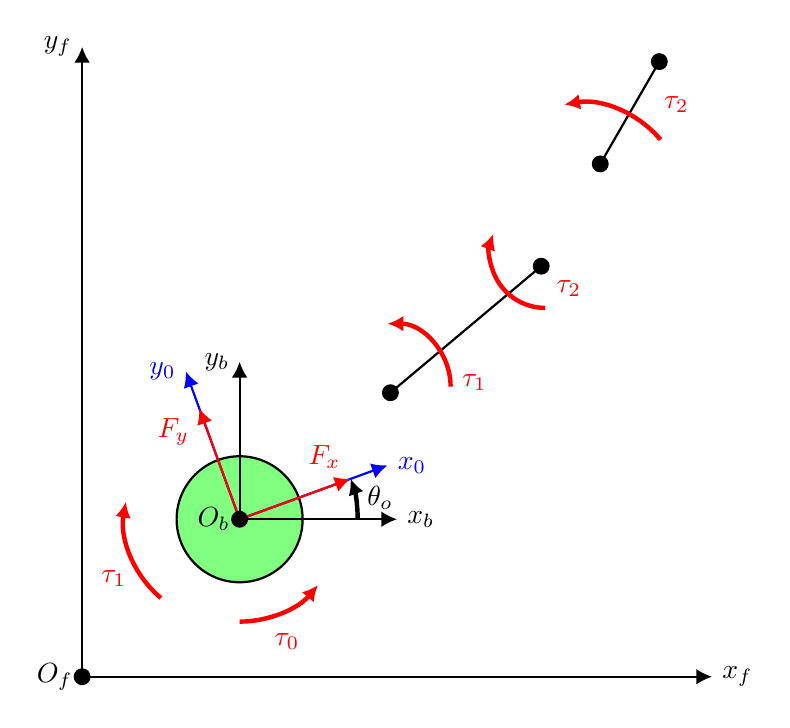
\begin{tikzpicture}

  \def\lone{5} 
  \def\ltwo{3}

  \def\thetazero{20}
  \def\thetaone{20}
  \def\thetatwo{20} 

  \coordinate (O) at (0,0);
  \coordinate (Ob) at (2,2);
  \coordinate (q) at (1,1);
  \coordinate (A') at ({2+\lone/2*cos(\thetaone+\thetazero)},{2+\lone/2*sin(\thetaone+\thetazero)});
  \coordinate (Ob0) at ({-0.2+3+2*cos(\thetazero)},{3+2*sin(\thetazero)});
  \coordinate (Ob00) at ({4+2*cos(\thetazero)},{4+2*sin(\thetazero)});
  \coordinate (Ob01) at ({-0.2+3+2*cos(\thetazero)},{-0.2+3+2*sin(\thetazero)});
  \coordinate (Ob02) at ({4+2*cos(\thetazero)},{4+2*sin(\thetazero)});
  \coordinate (A) at ({2+\lone*cos(\thetaone+\thetazero)},{2+\lone*sin(\thetaone+\thetazero)});
  \coordinate (C) at ({2+2*\lone*cos(\thetaone+\thetazero)},{2+2*\lone*sin(\thetaone+\thetazero)});
  \coordinate (C0) at ({1.6+1.5*\lone*cos(\thetaone+\thetazero)},{2+1.5*\lone*sin(\thetaone+\thetazero)});
  \coordinate (C01) at ({1.5+1.5*\lone*cos(\thetaone+\thetazero)},{2.2+1.5*\lone*sin(\thetaone+\thetazero)});
  \coordinate (B') at ({2+\lone*cos(\thetaone+\thetazero) + \ltwo/2*cos(\thetaone + \thetatwo+\thetazero)}, 
                      {2+\lone*sin(\thetaone+\thetazero) + \ltwo/2*sin(\thetaone + \thetatwo+\thetazero)});
  \coordinate (B) at ({2+\lone*cos(\thetaone+\thetazero) + \ltwo*cos(\thetaone + \thetatwo+\thetazero)}, 
                      {2+\lone*sin(\thetaone+\thetazero) + \ltwo*sin(\thetaone + \thetatwo+\thetazero)});
  \coordinate (B0) at ({3+1.5*\lone*cos(\thetaone+\thetazero) + 1.5*\ltwo*cos(\thetaone + \thetatwo+\thetazero)}, 
                      {3+1.5*\lone*sin(\thetaone+\thetazero) + 1.5*\ltwo*sin(\thetaone + \thetatwo+\thetazero)});

  \draw[thick,fill=green!50] (2,2) circle (0.8);

  \draw[thick, black] (A') -- (A);
  \draw[thick, black] (B') -- (B);

  \draw[thick,black,->] (O) -- (0,8) node[anchor=east]{$y_f$};
  \draw[thick,black,->] (O) -- (8,0) node[anchor=west]{$x_f$};

  \draw[thick,black,->] (Ob) -- (2,4) node[anchor=east]{$y_b$};
  \draw[thick,black,->] (Ob) -- (4,2) node[anchor=west]{$x_b$};

  \draw[thick,blue,->] (Ob) -- ({2-2*sin(\thetazero)},{2+2*cos(\thetazero)}) node[anchor=east]{$y_0$};
  \draw[thick,blue,->] (Ob) -- ({2+2*cos(\thetazero)},{2+2*sin(\thetazero)}) node[anchor=west]{$x_0$};

  \draw[thick,red,->] (Ob) -- ({2-1.5*sin(\thetazero)},{2+1.5*cos(\thetazero)}) node[anchor=north east]{$F_y$};
  \draw[thick,red,->] (Ob) -- ({2+1.5*cos(\thetazero)},{2+1.5*sin(\thetazero)}) node[anchor=south east]{$F_x$};
  

  \draw[ultra thick,->,red] (2,0.7) arc [start angle=-90, end angle=-40, x radius=1.3, y radius=1.3] node[anchor=south west] at (2.3,0.2) {$\tau_0$};
  \draw[ultra thick,->,red] (q) arc [start angle=-130, end angle=-190, x radius=1.3, y radius=1.3] node[anchor=south west] at (0.1,1) {$\tau_1$};
  \draw[ultra thick,->] (3.5,2) arc [start angle=0, end angle=\thetaone, x radius=1.5, y radius=1.5];
  \draw[ultra thick,->,red] (Ob0) arc [start angle=0, end angle={\thetaone+\thetazero+50}, x radius=0.8, y radius=0.8] node[anchor=south west] at (Ob01) {$\tau_1$};
  \draw[ultra thick,->,red] (Ob00) arc [start angle=-90, end angle=-200, x radius=0.7, y radius=0.7] node[anchor=south west] at (Ob02) {$\tau_2$};
  \draw[ultra thick,->, red] (C0) arc [start angle=\thetaone+20, end angle={\thetatwo+\thetaone+60}, x radius=1.3, y radius=1.3] node[anchor=south west] at (C01) {$\tau_2$};

  \filldraw[fill=black] (O) circle (0.1);
  \filldraw[fill=black] (Ob) circle (0.1);
  \filldraw[fill=black] (A') circle (0.1);
  \filldraw[fill=black] (A) circle (0.1);
  \filldraw[fill=black] (B) circle (0.1);
  \filldraw[fill=black] (B') circle (0.1);

  \node[anchor=east] at (O) {$O_f$};
  \node[anchor=east] at (Ob) {$O_b$};
  \node[anchor=south west] at (3.5,2) {$\theta_o$};

\end{tikzpicture}
  \caption{Forces and torques applied to the base ($F_x,F_y,\tau_0$) and to the links ($\tau_1,\tau_2$). Note that the torque of the first arm affects the base and the torque of the second arm affects the first arm.}
  \label{forces}
\end{figure}
In this case they are the torques and forces applied to the base and the manipulator's links (see Figure~\ref{forces}):
\begin{equation}
  \begin{array}{l}
  f_1=F_x\cos{\theta_0}-F_y\sin{\theta_0}\\
  f_2=F_x\sin{\theta_0}+F_y\cos{\theta_0}\\
  f_3=\tau_0\\
  f_4=\tau_1\\
  f_5=\tau_2
  \end{array}
  \label{non_lagrangian}
\end{equation}
Since the kinetic energy is written with respect to the fixed frame, the forces are projected too in that frame through $\theta_0$.\\
Equation (\ref{lagrangian}) can now be written as:
\begin{equation}
  \begin{cases}
    \frac{d}{dt}\frac{\partial \mathcal{L} }{\partial \dot{x}_b}-\frac{\partial \mathcal{L} }{\partial x_b}=F_x\cos{\theta_0}-F_y\sin{\theta_0}\\
    \frac{d}{dt}\frac{\partial \mathcal{L} }{\partial \dot{y}_b}-\frac{\partial \mathcal{L} }{\partial y_b}=F_x\sin{\theta_0}+F_y\cos{\theta_0}\\
    \frac{d}{dt}\frac{\partial \mathcal{L} }{\partial \dot{\theta}_0}-\frac{\partial \mathcal{L} }{\partial \theta_0}=\tau_0\\
    \frac{d}{dt}\frac{\partial \mathcal{L} }{\partial \dot{q}_1}-\frac{\partial \mathcal{L} }{\partial q_1}=\tau_1\\
    \frac{d}{dt}\frac{\partial \mathcal{L} }{\partial \dot{q}_2}-\frac{\partial \mathcal{L} }{\partial q_2}=\tau_2
  \end{cases}
\end{equation}
After having solved these five equations, it is possible to gather them together in a vectorial form, such as in (\ref{equation_motion}), with $M\in\mathbb{R}^{5\times 5}$, $C\in \mathbb{R}^5$ and $u\in\mathbb{R}^{5\times 5}$.\textcolor{red}{MATRICES IN THE APPENDIX?}
\subsection{Object's Dynamics}\label{object_dynamics}
The same approach can be implemented for the object to be captured: since it is approximated as a disk too, its moment of inertia is equal to the base's one.\\
The kinetic energy is then:
\begin{equation}
  T_O=v_Om_Ov_O^T+\frac{1}{2}I_{O_z}\theta_O^2
\end{equation}
and the non lagrangian components:
\begin{equation}
  \begin{array}{l}
  f_{O_1}=F_{O_x}\cos{\theta_O}-F_{O_y}\sin{\theta_O}\\
  f_{O_2}=F_{O_x}\sin{\theta_O}+F_{O_y}\cos{\theta_O}\\
  f_{O_3}=\tau_O
  \end{array}
\end{equation}
supposing to have, as the VMS' base, two translational forces acting on the centre of mass and a torque around its inertial frame. However, since we are not really interested in the control of the external object, these are not necessary and we will use only the mass and Coriolis matrices.\\
By solving equation (\ref{lagrangian}), we get the mass, Coriolis' and torques matrices:
\begin{equation}
  \begin{array}{c}
    M_O=\begin{bmatrix}
      m_O&0&0\\
      0&m_O&0\\
      0&0&\frac{m_Or^2}{2}
    \end{bmatrix}\quad
    C_O=\begin{bmatrix}
      0\\0\\0
    \end{bmatrix}\\
    \\
    u_O=\begin{bmatrix}
      \cos{\theta_O}&-\sin{\theta_0}&0\\
      \sin{\theta_O}&\cos{\theta_0}&0\\
      0&0&1
    \end{bmatrix}
  \end{array}
  \label{object_matrices}
\end{equation}
\newpage
\section{Homogeneous Matrices Approach}
The Homogeneous Matrices Approach introduced in [9,10] offers a quick, intuitive and scalable (for higher DoFs) method for robotic's dynamics.\\
It is base, as the name suggests, on the Homogeneous Matrices shown in Section~\ref{Homogeneous} and on other characteristic matrices that will be here presented.\\
The goal of this approach is to write the lagrangian in a matrix form and, to do so, we need to define matrices for the inertia of the system, for the non-lagrangian actions present in the system and the velocity of the bodies.\\
The latter ones have already been discussed in Section~\ref{velocity_section}, while the inertia and non-lagrangian forces need to be introduced.\\

The mass distribution of a body $k$, projected in the frame $i$, can be described through the \textit{Pseudo Inertia Tensor} $J$:
\begin{equation}
  \prescript{i}{}{J_k}=\begin{bmatrix}
    J_{xx}&J_{xy}&J_{xz}&mx_G\\
    J_{yx}&J_{yy}&J_{yz}&my_G\\
    J_{zx}&J_{zy}&J_{zz}&mz_G\\
    mx_G&my_G&mz_G&m
  \end{bmatrix}
\end{equation}
where $m$ is the mass of the body, $\{x_G,y_G,z_G\}$ is the position of the centre of mass and the pseudo moments of inertia are defined as:
\begin{equation}
  \begin{array}{c}
    J_{xx}=\int x^2\,dm\quad J_{yy}=\int y^2\,dm\quad J_{zz}=\int z^2\,dm\\
    J_{xy}=\int xy\,dm\quad J_{xz}=\int xz\,dm\quad J_{yz}=\int yz\,dm
  \end{array}
  \label{pseudo_moments}
\end{equation}
These are differents from the well known moments of inertia ($I_{xx},I_{yy},I_{zz},I_{xy},I_{xz},I_{yz}$) and their relation is shown in equation (\ref{moments_convertion}):
\begin{equation}
  \begin{array}{c}
    \begin{cases}
      J_{xx}=\frac{-I_{xx}+I_{yy}+I_{zz}}{2}\\
      J_{yy}=\frac{-I_{yy}+I_{xx}+I_{zz}}{2}\\
      J_{zz}=\frac{-I_{zz}+I_{xx}+I_{yy}}{2}
    \end{cases}
    \quad
    \begin{cases}
      J_{xy}=-I_{xy}\\
      J_{yz}=-I_{yz}\\
      J_{zz}=-I_{zx}
    \end{cases}
  \end{array}
\label{moments_convertion}
\end{equation}
\\
In order to evaluate the non lagrangian components of equation (\ref{lagrangian}), [9] introduces the \textit{Action Matrix}:
\begin{equation}
  \prescript{i}{}{\phi}_k=\begin{bmatrix}
    0&-c_z&c_y&f_x\\
    c_z&0&-c_x&f_y\\
    -c_y&c_x&0&f_z\\
    -f_x&-f_y&-f_z&0
  \end{bmatrix}
  \label{action_matrix}
\end{equation}
where $\{f_x,f_y,f_z\}$ is the resultant of the forces applied to a body $k$, $\{c_x,c_y,c_z\}$ holds the torques calculated with respect to the origin of the frame $i$.\\
The pseudo-scalar product (see \ref{appendix}) between the action matrix of a body and its velocity matrix, gives the power developed by the actions included in $\phi$ as the object moves according to the velocities described by $W$:
\begin{equation}
  P=\prescript{f}{}{\phi}\otimes \prescript{f}{}{W}
\end{equation}
Notice that both the action and velocity matrix have been projected in the fixed frame.\\
A manipulator with two revolute links will have two contribution to the overall power, one for each link:
\begin{equation}
  \begin{split}
  P&=\prescript{f}{}{\phi_1}\otimes \prescript{f}{}{W_{f1}}+\prescript{f}{}{\phi_2}\otimes \prescript{f}{}{W_{f2}}\\
   &=\prescript{f}{}{\phi_1}\otimes \prescript{f}{}{L_{f1}}\dot{\theta_1}+\prescript{f}{}{\phi_2}\otimes \Big(\prescript{f}{}{W_{f1}}+\prescript{f}{}{W_{12}}\Big)\\
   &=\Big(\prescript{f}{}{\phi_1}+\prescript{f}{}{\phi_2}\Big)\otimes\prescript{f}{}{L_{f1}}\dot{\theta_1}+\prescript{f}{}{\phi_2}\otimes \prescript{f}{}{L_{12}}\dot{\theta_2}\\
   &=f_{\theta_1}\dot{\theta_1}+f_{\theta_2}\dot{\theta_2}
  \end{split}
\end{equation}
whith $f_{\theta_1}$ and $f_{\theta_2}$ the non-lagrangian components of links one and two, respectively.\\
It is now clear the importance of the $L$ matrix, introduced in Section~\ref{velocity_section}: we can write the non-lagrangian components as a pseudo-scalr product between the overall set of action applied to the system downstream and the relative motion permitted by the joint $i$:
\begin{equation}
  f_{q_i}=\Big(\sum_{j=1}^N\prescript{f}{}{\phi_j}\Big)\otimes \prescript{f}{}{L_{q_i}}
\label{non_lagrangian_matrix}
\end{equation}
It can be proved that ideal constraints between links don't affect the Lagrange equation: we can neglet the constraint forces in $\phi$.\\

Finally, we can write the kinetic energy of the body $j$ as follows:
\begin{equation}
  T_j=\frac{1}{2}\Tr{\Big(\prescript{f}{}{W_{fj}}\prescript{f}{}{J_j}\prescript{f}{}{W_{fj}^T}\Big)}
  \label{kinetic_matrix}
\end{equation}
and, from equation (\ref{energy_sum}), we still get (\ref{lagrangian}).\\

Regarding the planar VMS system, it is useful to write the pseudo inertial tensor starting from the local frame: since the body is rigid, the mass is supposed to remain in the same position with respect to the local frame.\\
The pseudo moments of inertia are found starting from the moments of inertia (Table \ref{inertia_moments}) and following equation (\ref{moments_convertion}), as shown in Table~\ref{pseudo_moments_table}. Thus:
\begin{equation}
  \begin{array}{c}
  \prescript{0}{}{J_b}=\begin{bmatrix}
    \frac{m_br^2}{4}&0&0&0\\
    0&\frac{m_br^2}{4}&0&0\\
    0&0&0&0\\
    0&0&0&m_b
  \end{bmatrix} \quad
    \prescript{1}{}{J_1}=\begin{bmatrix}
    \frac{l_1^2m_1}{3}&0&0&0\\
    0&0&0&-\frac{l_1m_1}{2}\\
    0&0&0&0\\
    \frac{l_1m_1}{2}&0&0&m_1
  \end{bmatrix}\\
  \\
  \prescript{2}{}{J_2}=\begin{bmatrix}
    \frac{l_2^2m_2}{3}&0&0&0\\
    0&0&0&-\frac{l_2m_2}{2}\\
    0&0&0&0\\
    \frac{l_2m_2}{2}&0&0&m_2
  \end{bmatrix}
  \end{array}
\end{equation}
\begin{table}
  \caption{Moments of inertia of the planar VMS' bodies, with respect to their centre of mass (in the centre of the base and the arms), with $i=\{1,2\}$.}
  \label{pseudo_moments_table}
  \begin{center}
  \begin{tabular}{lccc}
    \toprule
  \textbf{Body} & \textbf{Tensor of Pseudo Inertia}\\
  \midrule
  Base&$\begin{bmatrix}
    \frac{1}{4}m_br^2&0&0\\
    0&\frac{1}{4}m_br^2&0\\
    0&0&0
  \end{bmatrix}$\\
  \\
  Arms&$\begin{bmatrix}
    \frac{1}{3}m_il_i^2&0&0\\
    0&0&0\\
    0&0&0
  \end{bmatrix}$\\
  \bottomrule
  \end{tabular}
  \end{center}
  \end{table}
Then, following equation (\ref{change_frame}), we can project $\prescript{0}{}{J_b}$, $\prescript{1}{}{J_1}$ and $\prescript{2}{}{J_2}$ in the fixed frame, obtaining $\prescript{f}{}{J_b}$, $\prescript{f}{}{J_1}$ and $\prescript{f}{}{J_2}$.\\
It is already possibile to write the kinetic energy (\ref{kinetic_matrix}) for every body, since we have both the velocity matrices and the tensors of pseudo inertia projected in the fixed frame:
\begin{equation}
  \begin{array}{l}
    T_b=\frac{1}{2}\Tr{\Big(\prescript{f}{}{W_{f0}}\prescript{f}{}{J_0}\prescript{f}{}{W_{f0}^T}\Big)}\\
    T_1=\frac{1}{2}\Tr{\Big(\prescript{f}{}{W_{f1}}\prescript{f}{}{J_1}\prescript{f}{}{W_{f1}^T}\Big)}\\
    T_2=\frac{1}{2}\Tr{\Big(\prescript{f}{}{W_{f2}}\prescript{f}{}{J_2}\prescript{f}{}{W_{f2}^T}\Big)}
  \end{array}
\end{equation}
To find the non lagrangian components, the action and the $L$ matrices need to be calculated.\\
We have already found the $L$ matrices associated with the permitted motion of each body in Chapter~\ref{kinematics} (see equation (\ref{L_matrices})). The action matrices can be easily found by looking at the definition of $\phi$ (\ref{action_matrix}) and confronting it with Figure~\ref{forces}:
\begin{equation}
  \begin{array}{c}
    \prescript{0}{}{\phi_b}=\begin{bmatrix}
      0&-\tau_0+\tau_1&0&F_x\\
      \tau_0-\tau_1&0&0&F_y\\
      0&0&0&0\\
      -F_x&-F_y&0&0
    \end{bmatrix} \quad
    \prescript{1}{}{\phi_1}=\begin{bmatrix}
      0&-\tau_1+\tau_2&0&0\\
      \tau_1-\tau_2&0&0&0\\
      0&0&0&0\\
      0&0&0&0
    \end{bmatrix}\\
    \\
    \prescript{2}{}{\phi_2}=\begin{bmatrix}
      0&-\tau_3&0&0\\
      \tau_2&0&0&0\\
      0&0&0&0\\
      0&0&0&0
    \end{bmatrix}
  \end{array}
\end{equation}
After the projection of the action matrices in the fixed frame, it is possible to find the non lagrangian components:
\begin{equation}
  \begin{array}{l}
  f_1=\Big(\prescript{f}{}{\phi_b}+\prescript{f}{}{\phi_1}+\prescript{f}{}{\phi_2}\Big)\otimes \prescript{f}{}{L_{fb_x}}=F_x\cos{\theta_0}-F_y\sin{\theta_0}\\
  f_2=\Big(\prescript{f}{}{\phi_b}+\prescript{f}{}{\phi_1}+\prescript{f}{}{\phi_2}\Big)\otimes \prescript{f}{}{L_{fb_y}}=F_x\sin{\theta_0}+F_y\cos{\theta_0}\\
  f_3=\Big(\prescript{f}{}{\phi_b}+\prescript{f}{}{\phi_1}+\prescript{f}{}{\phi_2}\Big)\otimes \prescript{f}{}{L_{f0}}=\tau_0\\
  f_4=\Big(\prescript{f}{}{\phi_b}+\prescript{f}{}{\phi_1}\Big)\otimes \prescript{f}{}{L_{01}}=\tau_1\\
  f_5=\prescript{f}{}{\phi_b}\otimes \prescript{f}{}{L_{12}}=\tau_2
  \end{array}
\end{equation}
which are the same of (\ref{non_lagrangian}).\\
It is now possibile to solve the Lagrange equation, 
with $\mathcal{L}=T_b+T_1+T_2$:
\begin{equation}
  \begin{cases}
    \frac{d}{dt}\frac{\partial \mathcal{L} }{\partial \dot{x}_b}-\frac{\partial \mathcal{L}}{\partial x_b}=f_1\\
    \frac{d}{dt}\frac{\partial \mathcal{L} }{\partial \dot{y}_b}-\frac{\partial \mathcal{L}}{\partial y_b}=f_2\\
    \frac{d}{dt}\frac{\partial \mathcal{L} }{\partial \dot{\theta}_0}-\frac{\partial \mathcal{L}}{\partial \theta_0}=f_3\\
    \frac{d}{dt}\frac{\partial \mathcal{L} }{\partial \dot{q}_1}-\frac{\partial \mathcal{L}}{\partial q_1}=f_4\\
    \frac{d}{dt}\frac{\partial \mathcal{L} }{\partial \dot{q}_2}-\frac{\partial \mathcal{L}}{\partial q_2}=f_5\\
  \end{cases}
\end{equation}
\subsection{Object's Dynamics}
The object's pseudo inertia tensor follows the same structure of the base's one:
\begin{equation}
  \prescript{O_1}{}{J_{O_1}}=\begin{bmatrix}
    \frac{m_br^2}{4}&0&0&0\\
    0&\frac{m_br^2}{4}&0&0\\
    0&0&0&0\\
    0&0&0&m_b
  \end{bmatrix}
\end{equation}
and $\prescript{f}{}{J_b}=\prescript{f}{O_1}{M}\prescript{O_1}{}{J_{O_1}}\prescript{O_1}{f}{M}$.\\
The velocity and $L$ matrices have already been found in the previous chapter; the action matrix can be written with the same assimption made for the classic method approach:
\begin{equation}
  \prescript{O_1}{}{\phi_{O_1}}=\begin{bmatrix}
    0&-\tau_O&0&F_{O_x}\\
    \tau_O&0&0&F_{O_y}\\
    0&0&0&0\\
    -F_{O_x}&-F_{O_y}&0&0
  \end{bmatrix}
\end{equation}
and $\prescript{f}{}{\phi_{O_1}}=\prescript{f}{O_1}{M}\prescript{O_1}{}{\phi_{O_1}}\prescript{O_1}{f}{M}$.
Finally:
\begin{equation}
  T_O=\frac{1}{2}\Tr{\Big(\prescript{f}{}{W_{fO_1}}\prescript{f}{}{J_b}\prescript{f}{}{W_{fO_1}^T}\Big)}
\end{equation}
and:
\begin{equation}
  \begin{array}{l}
    f_{O_1}=\prescript{f}{}{\phi_{O_1}}\otimes \prescript{f}{}{L_{fO_x}}=F_{O_x}\cos{\theta_O}-F_{O_y}\sin{\theta_O}\\
    f_{O_2}=\prescript{f}{}{\phi_{O_1}}\otimes \prescript{f}{}{L_{fO_y}}=F_{O_y}\cos{\theta_O}+F_{O_x}\sin{\theta_O}\\
    f_{O_3}=\prescript{f}{}{\phi_{O_1}}\otimes \prescript{f}{}{L_{O_0O_1}}=\tau_O
  \end{array}
\end{equation}
By solving (\ref{lagrangian}), we get the same matrices in (\ref{object_matrices}).
\newpage
\chapter{Impact Analysis}\label{impact_analysis}
Once the Kinematics and the Dynamics of both the VMS and the external object are analysed, the impact analysis between the two is here performed.\\
In [13] and [14], two basic assumptions are made in the formulation of the impact model:
\begin{enumerate}
  \item although the generalized velocities change substantially, the generalized coordinates of the system remain the same over the impact duration. This is justified not only for the rotational coordinates but for the elastic ones as well [15]. The latter conclusion can also be implied by reasoning that since the duration of impact (approximately \SI{d-4}{\second}) is very small compared with the period of the fundamental mode of vibration of the links (several seconds), the change in deflection of a flexible beam during impact is negligible;
  \item at the contact point between the end-defector and the target there are forces but not moments. Impact occurs at a single point, which is unable to transmit a local moment.
\end{enumerate}
Another assumption that has been already done in the previous chapters is that we know in advance the inertia and dynamic properties of the payload, as well as the position of the contact point on the payload.\\
Following the second assumption, during the impact the equations of motion of the VMS and the object can be expressed in a form similar to equation (\ref{equation_motion}) except for the impact force $f_I$:
\begin{equation}
  \begin{cases}
    M\ddot{p}+C=u+J^Tf_I\\
    M_O\ddot{\psi}+C_O=-J_O^Tf_I
  \end{cases}
  \label{initial_impact}
\end{equation}
where $J^Tf_I$ and $J_O^Tf_I$ are the torques and forces applied to the VMS and object's generalized coordinates respectively, following the relation shown in (\ref{force_jacobian}). For the second assumption, the wrench is now composed of the force $f_I$ only.\\
Notice that $u_O$ has been omitted in the second equation, since, as already mentioned in Section~\ref{object_dynamics}, we are not interested in controlling the object.\\
From the second equation of (\ref{initial_impact}), we can write:
\begin{equation}
  f_I=-(J_O^T)^+(M_O\ddot{\psi}_O+C_O)
  \label{impact_force}
\end{equation}
with $(J_O^T)^+$ the pseudoinverse of the transposed object's jacobian; in fact, since as found in (\ref{object_jacobian}) this jacobian is not squared, we can use the pseudoinverse to invert it and, by having linearly indipendent rows, it is defined accordingly to (\ref{pseudoinverse}).\\
By substuting (\ref{impact_force}) in the first equation of (\ref{initial_impact}), one obtaines:
\begin{equation}
  \begin{split}
  M\ddot{p}+C&=u-J^T(J_O^T)^+(M_O\ddot{\psi}_O+C_O)\\
  &=u-J^T(J_O^+)^T(M_O\ddot{\psi}_O+C_O)
  \end{split}
\end{equation}
Now, integrating the above equation over the period od impact $\pi$:
\begin{equation}
  \int_{0}^{\pi}M\ddot{p}\,dt+\int_{0}^{\pi}C\,dt =-\int_{0}^{\pi}J^T(J_O^+)^TM_O\ddot{\psi}_O\,dt+\int_{0}^{\pi}(u-J^T(J_O^+)^TC_O)\,dt
\end{equation}
Under the first assumption of no change of the generalized coordinates during the impact (but only of their velocities), all the contributions that depend only on the velocities and positions (i.e. $C,u,J^T(J_O^+)^TC_O$) can be ignored:
\begin{equation}
  M(\dot{p}_f-\dot{p}_i)+J^T(J_O^+)^TM_O(\dot{\psi}_f-\dot{\psi_i})=0
  \label{general_impact}
\end{equation}
This equation can be used for all collisions ranging from plastic to perfectly elastic~[15,16]. It is in fact the general property of conservation of momentum:  given two point masses $m_1$ and $m_2$, with linear initial velocity $v_{1,i}$ and $v_{2,i}$, the conservation of momentum law states:
\begin{equation}
  m_1v_{i,1}+m_2v_{i,2}=m_1v_{f,1}+m_2v_{f,2}
\end{equation}
or, equivalently:
\begin{equation}
  m_1(v_{f,1}-v_{i,1})+m_2(v_{f,2}-v_{i,2})=0
  \label{momentum_conservation}
\end{equation}
Equation (\ref{momentum_conservation}) is very similar to (\ref{general_impact}), with the difference that $M\dot{p}\in \mathbb{R}^{5\times 1}$ and $M_O\dot{\psi}\in \mathbb{R}^{3\times 1}$: they cannot be summed. That is why the object's mass matrix is multiply by the two jacobians, which comes directly from the equation of motion.\\
In the following sections two different scenarios will be analysedby assuming the manipulator's arms as rigid or elastic bodies.
\newpage
\section{Rigid Bodies}\label{rigid}
In a plastic impact, the velocity of the contact point of each system is the same after the impact:
\begin{equation}
  J\dot{p_f}=J_O\dot{\psi_f}
  \label{kinematic_constraint}
\end{equation}
where the left-hand side term of the equation is the velocity of the contact point written as a function of the final VMS generalized coordinates and velocities $p_f,\dot{p}_f$ (see (\ref{task_dimension})) and the right-hand side term is the velocity of the same point written with respect to the object generalized final coordinates and velocities $\psi_f,\dot{\psi}_f$.\\
From (\ref{kinematic_constraint}), the velocities of the object can be expressed in terms of those of the VMS as:
\begin{equation}
  \dot{\psi}_f=J_O^+J\dot{p}_f
  \label{composition}
\end{equation}
By substituting equation (\ref{composition}) in equation (\ref{general_impact}), the following is obtained:
\begin{equation}
  \dot{p}_f=G^{-1}H
  \label{final_velocities}
\end{equation}
where:
\begin{equation}
  \begin{array}{l}
    G=M+J^T(J_O^+)^TM_OJ_O^+J\\
    H=M\dot{p}_i+J^T(J_O^+)^TM_O\dot{\psi}_i
  \end{array}
\end{equation}
We can confront this result with the one obtained starting from equation (\ref{momentum_conservation}) in the case of two point masses; since the final velocity in a plastic impact would have been the same $v_f$ for both masses, we can write:
\begin{equation}
  \begin{array}{l}
  m_1v_{i,1}+m_2v_{i,2}=(m_1+m_2)v_f\\
  \Rightarrow v_f=g^{-1}h
  \end{array}
\end{equation}
with:
\begin{equation}
  \begin{array}{l}
    g=m_1+m_2\\
    h=m_1v_{i,1}+m_2v_{i,2}
  \end{array}
\end{equation}
Notice that $G,H$ are very similar to $g,h$, the difference is still due to the jacobians matrices which come from the kinematic relation.\\
Once the initial velocities $\dot{p}_i,\dot{\psi}_i$ have been determined, $\dot{p}_f$ can be evaluated according to (\ref{final_velocities}) and $\dot{\psi}_f$ can be solved from (\ref{composition}). These final values are used as the initial velocity conditions for the post-impact dynamical simulation of the system, whose model will be the combination of the equations of robot and object, so that equation (\ref{composition}) will always hold and we can get rid off the subscripts:
\begin{equation}
  \dot{\psi}=J_O^+J\dot{p}
\end{equation}
While in [14] the post-impact analyisis is not fully covered, [16] offers an intuitive procedure to write the dynamics of the new VMS, composed now by the object too, with respect of the VMS generalized coordinates alone (i.e. $p$).\\ 
By differentiating the above equation we can obtain:
\begin{equation}
  \ddot{\psi}=J_O^+J\ddot{p}+\frac{\partial J_O^+}{\partial t}J\dot{p}+J_O^+\frac{\partial J}{\partial t}\dot{p}
  \label{composition_diff}
\end{equation}
We can now substitute (\ref{composition_diff}) in the second equation of (\ref{initial_impact}) (i.e. the dynamics of the object), obtaining:
\begin{equation}
  M_O\Big(J_O^+J\ddot{p}+\frac{\partial J_O^+}{\partial t}J\dot{p}+J_O^+\frac{\partial J}{\partial t}\dot{p}\Big)+C_O=-J_O^Tf_I
\end{equation}
from which $f_I$ can be written as:
\begin{equation}
  f_I=-\Big(J_O^{-T}M_OJ_O^+J\ddot{p}+J_O^{-T}M_O\frac{\partial J_O^+}{\partial t}J\dot{p}+J_O^{-T}M_OJ_O^+\frac{\partial J}{\partial t}\dot{p}+J_O^{-T}C_O\Big)
\end{equation}
Now, $f_I$ can be substituted in the first equation of (\ref{initial_impact}) (i.e. the VMS dynamics) and by doing so, we can write the overall dynamics with respect to $p$ only:
\begin{equation}
  M'\ddot{p}+C'=u
  \label{final_equation_motion}
\end{equation}
where:
\begin{equation}
  \begin{array}{l}
    M'=M+J^T(J_O^T)^+M_OJ_O^+J\\
    C'=C+J^T(J_O^T)^+M_O\frac{\partial J_O^+}{\partial t}J\dot{p}+J^T(J_O^T)^+M_OJ^+\frac{\partial J}{\partial t}\dot{p}+J^T(J_O^T)^+C_O
  \end{array}
  \label{VMS_dynamics}
\end{equation}
Equation (\ref{VMS_dynamics}) is the post-impact dynamic model of the VMS containing the object. Both $M'$ and $C'$ are still dependent on $J_O$, which depends on the object's coordinates, but since the object is now captured by the manipulator, its coordinated coincide with the end-effector ones, and its velocities are found by differentization.
\newpage
\FloatBarrier
\subsection{Free Motion}
A simulation has been perfomed by means of the Mathematica software (version 13.2.1.0) with VMS paramers shown in Table~\ref{VMS_parameters} and the initial conditions shown in Tables~\ref{initial_positions}, \ref{initial_velocities}.\\
The VMS parameters have been chosen following a real case scenario: the lenghts, radiuses and masses of the manipulator's arms are the ERA ones (see Table~\ref{SRMs_comparison} and [4]); the base mass is the mass of the ISS, on top of which the ERA is attached; the payload mass is the mass of a medium-size satellite; $\gamma$ is an arbitrary value.\\
Regarding the VMS initial positions, the choice of the values will be explained in the next section. For this analysis, every initial position is valid. The initial velocities are zero for almost every VMS generalized coordinate (i.e we assume the base and manipulator still before the impact) and small initial velocities for the payload, as the case of satellite docking is taken into consideration: the ideal condition would be a null relative velocities, however, in a real case scenario, a non-zero relative veloties is present.\\
\begin{table}
  \caption{VMS parameters.}
  \label{VMS_parameters}
  \begin{center}
  \begin{tabular}{cccccccc}
    \toprule
    $l_1$&$l_2$&$m_b$&$m_1$&$m_2$&$m_O$&$r$&$\gamma$\\
  \midrule
    \SI{5.59}{\metre}&\SI{5.59}{\metre}&\SI{419725}{\kilogram}&\SI{300}{\kilogram}&\SI{300}{\kilogram}&\SI{3000}{\kilogram}&\SI{0.12}{\metre}&\SI{0.5}{\radian}\\
  \bottomrule
  \end{tabular}
  \end{center}
\end{table}
\begin{table}
  \caption{Simulation's initial positions.}
  \label{initial_positions}
  \begin{center}
  \begin{tabular}{cccccccc}
    \toprule
    $x_b$&$y_b$&$\theta_0$&$q_1$&$q_2$&$x_O$&$y_O$&$\theta_O$\\
  \midrule
    \SI{4}{\metre}&\SI{2}{\metre}&\SI[parse-numbers = false]{\pi/2}{\radian}&\SI{0}{\radian}&\SI[parse-numbers = false]{\pi/2}{\radian}&\SI{-1.71}{\metre}&\SI{7.59}{\metre}&\SI{5.78}{\radian}\\
  \bottomrule
  \end{tabular}
  \end{center}
\end{table}
\begin{table}
  \caption{Simulation's initial velocities.}
  \label{initial_velocities}
  \begin{center}
  \begin{tabular}{lcc}
    \toprule
    &\textbf{Simulation 1}&\textbf{Simulation 2}\\
  \midrule
  $\dot{\theta_0}$&\SI{0}{\radian\per\second}&\SI{0}{\radian\per\second}\\
  $\dot{x_b}$&\SI{0}{\metre\per\second}&\SI{0}{\metre\per\second}\\
  $\dot{y_b}$&\SI{0}{\metre\per\second}&\SI{0}{\metre\per\second}\\
  $\dot{q_1}$&\SI{0}{\radian\per\second}&\SI{0}{\radian\per\second}\\
  $\dot{q_2}$&\SI{0}{\radian\per\second}&\SI{0}{\radian\per\second}\\
  $\dot{x_O}$&\SI{-0.1}{\metre\per\second}&\SI{0}{\metre\per\second}\\
  $\dot{y_O}$&\SI{0}{\metre\per\second}&\SI{-0.1}{\metre\per\second}\\
  $\dot{\theta}_O$&\SI{0.01}{\radian\per\second}&\SI{0.01}{\radian\per\second}\\
  \bottomrule
  \end{tabular}
  \end{center}
\end{table}
The position of the object in the pre-impact has been found by imposing that the contact point coincides with the initial end-effector position, while its orientation $\theta_O$ has been chosen as follows:
\begin{equation}
  \theta_O=\theta_{0,0}+q_{1,0}+q_{2,0}+\pi-\gamma
  \label{contact_rotation}
\end{equation}
which is, the orientation of the object is such that it is rotated of the same end-effector angle ($\theta_{0,0}+q_{1,0}+q_{2,0}$) minus $\gamma$ to align the x-axis with the EE's one. In order to make the contact point coincide with the EE, \SI{180}{\degree} have been added.\\
As shown in Table~\ref{initial_velocities}, two simulations have been performed, with the only difference in the object's initial velocities: in the first simulation, the payload moved only in the negative x-direction, in the second it moves only in the negative y-direction.\\
Given these initial conditions, the final velocities $\dot{p}_f$ in (\ref{final_velocities}) can be calculated.\\

For the post-impact analysis, the position of the object have been imposed again as a function of the EE position, but now as a function of time, and its orientation similarly to equation (\ref{contact_rotation}):
\begin{equation}
  \theta_O(t)=\theta_0(t)+q_1(t)+q_2(t)+\pi-\gamma
\end{equation}
Having now the new post-impact $\psi_p$ generalized coordinates as a function of $p$, the object's jacobian can be expressed as a function of the VMS generalized coordinates too and $M'$ and $C'$ can be found according to (\ref{VMS_dynamics}).\\
A control-free dynamics has been performed using as inital conditions the initial positions in Table~\ref{initial_positions} and the final velocities $\dot{p}_f$ found in the pre-impact analysis. As already stated at the beginning of this chapter, in fact, during the impact only the rates change, while the positions remain the same.\\
A quick and intuitive visual result can be seen in Figure~\ref{no_control_result}, while the evolution of the generalized coordinates over time are reported in Figures~\ref{free_motion_1}, \ref{free_motion_2}.\\
It is interesting to notice that, in both cases, $\theta_0$ does not change over time: the absence of a torque applied to the base allows free rotation of $q_1$ around $z_b$, since the manipulator is directly attached to the CoM of the base (i.e. the arm does not apply any torque) and the base does not rotate.\\
Furthermore, given the higher mass of the base with respect to the payload and manipulator masses, it moves very little and we can approximate it as still in the next calculations.\\
\begin{figure}[!htb]
  \centering
  \subfloat[][\emph{Simulation 1.}]
  {\scalebox{0.8}{
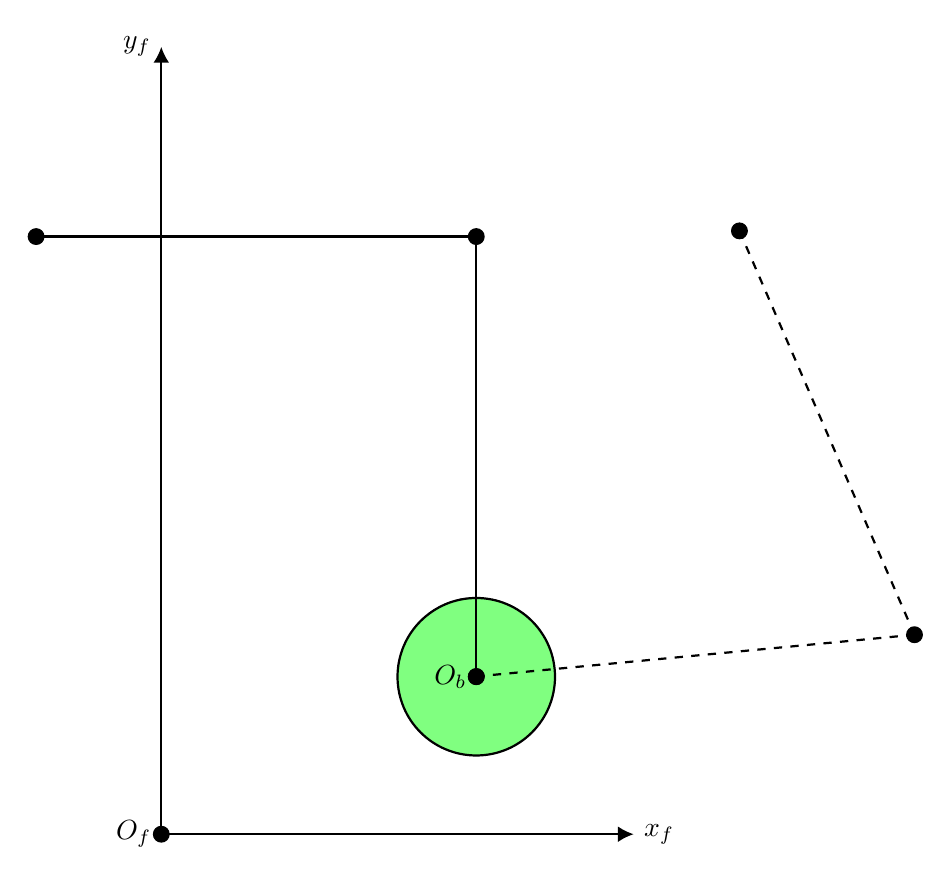
\begin{tikzpicture}

  \def\lone{5.59} 
  \def\ltwo{5.59}

  \def\thetazero{90}
  \def\thetaone{0}
  \def\thetatwo{90} 

  \coordinate (O) at (0,0);
  \coordinate (Ob) at (4,2);
  \coordinate (A) at ({4+\lone*cos(\thetaone+\thetazero)},{2+\lone*sin(\thetaone+\thetazero)});
  \coordinate (B) at ({4+\lone*cos(\thetaone+\thetazero) + \ltwo*cos(\thetaone + \thetatwo+\thetazero)}, 
                      {2+\lone*sin(\thetaone+\thetazero) + \ltwo*sin(\thetaone + \thetatwo+\thetazero)});
  \coordinate (Obp) at (4.00068, 2.00333);
  \coordinate (Ap) at (9.56548, 2.53356);
  \coordinate (Bp) at (7.34235, 7.66248);

  \draw[dashed,fill=green!25] (Obp) circle (1);
  \draw[thick,fill=green!50] (Ob) circle (1);

  \draw[thick, black] (Ob) -- (A);
  \draw[thick, black] (A) -- (B);
  \draw[thick, black, dashed] (Obp) -- (Ap);
  \draw[thick, black, dashed] (Ap) -- (Bp);

  \draw[thick,black,->] (O) -- (0,10) node[anchor=east]{$y_f$};
  \draw[thick,black,->] (O) -- (6,0) node[anchor=west]{$x_f$};

  \filldraw[fill=black] (O) circle (0.1);
  \filldraw[fill=black] (Ob) circle (0.1);
  \filldraw[fill=black] (A) circle (0.1);
  \filldraw[fill=black] (B) circle (0.1);
  \filldraw[fill=black] (Obp) circle (0.1);
  \filldraw[fill=black] (Ap) circle (0.1);
  \filldraw[fill=black] (Bp) circle (0.1);

  \node[anchor=east] at (O) {$O_f$};
  \node[anchor=east] at (Ob) {$O_b$};

\end{tikzpicture}}}
\subfloat[][\emph{Simulation 2.}]
  {\scalebox{0.8}{
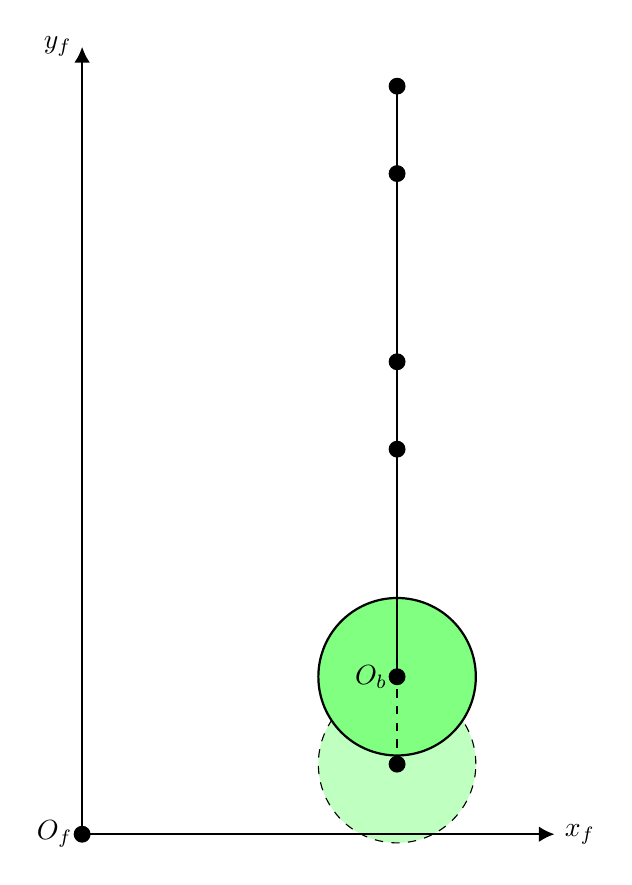
\begin{tikzpicture}

  \def\lone{4} 
  \def\ltwo{3.5}

  \def\thetazero{90}
  \def\thetaone{0}
  \def\thetatwo{0} 

  \coordinate (O) at (0,0);
  \coordinate (Ob) at (4,2);
  \coordinate (A) at ({4+\lone*cos(\thetaone+\thetazero)},{2+\lone*sin(\thetaone+\thetazero)});
  \coordinate (B) at ({4+\lone*cos(\thetaone+\thetazero) + \ltwo*cos(\thetaone + \thetatwo+\thetazero)}, 
                      {2+\lone*sin(\thetaone+\thetazero) + \ltwo*sin(\thetaone + \thetatwo+\thetazero)});
  \coordinate (Obp) at (4,0.89);
  \coordinate (Ap) at (4,4.89);
  \coordinate (Bp) at (4,8.39);

  \draw[dashed,fill=green!25] (Obp) circle (1);
  \draw[thick,fill=green!50] (Ob) circle (1);

  \draw[thick, black] (Ob) -- (A);
  \draw[thick, black] (A) -- (B);
  \draw[thick, black, dashed] (Obp) -- (Ap);
  \draw[thick, black, dashed] (Ap) -- (Bp);

  \draw[thick,black,->] (O) -- (0,10) node[anchor=east]{$y_f$};
  \draw[thick,black,->] (O) -- (6,0) node[anchor=west]{$x_f$};

  \filldraw[fill=black] (O) circle (0.1);
  \filldraw[fill=black] (Ob) circle (0.1);
  \filldraw[fill=black] (A) circle (0.1);
  \filldraw[fill=black] (B) circle (0.1);
  \filldraw[fill=black] (Obp) circle (0.1);
  \filldraw[fill=black] (Ap) circle (0.1);
  \filldraw[fill=black] (Bp) circle (0.1);

  \node[anchor=east] at (O) {$O_f$};
  \node[anchor=east] at (Ob) {$O_b$};

\end{tikzpicture}}} 
  \caption{Initial and final (dashed) position of the VMS after the impact for the two different simulations. In the left image, the satellite approaches the VMS with a west to east motion, while in the right one with a north to south motion.}
  \label{no_control_result}
\end{figure}
\begin{figure}[!htb]
  \centering
  \subfloat
  {\includesvg[scale=0.37]{free_motion_x.svg}} \quad
\subfloat
  {\includesvg[scale=0.37]{free_motion_y.svg}} \\
  \subfloat
  {\includesvg[scale=0.37]{free_motion_theta.svg}} \quad
  \subfloat
  {\includesvg[scale=0.37]{free_motion_q1.svg}}\\
  \subfloat
  {\includesvg[scale=0.37]{free_motion_q2.svg}}
  \caption{VMS generalized coordinates' displacement after the catching of the payload when no control is performed, simulation one.}
  \label{free_motion_1}
\end{figure}
\begin{figure}[!htb]
  \centering
  \subfloat
  {\includesvg[scale=0.37]{free_motion_x2.svg}}\quad
\subfloat
  {\includesvg[scale=0.37]{free_motion_y2.svg}} \\
  \subfloat
  {\includesvg[scale=0.37]{free_motion_theta2.svg}}\quad
  \subfloat
  {\includesvg[scale=0.37]{free_motion_q12.svg}}\\
  \subfloat
  {\includesvg[scale=0.37]{free_motion_q22.svg}}
  \caption{VMS generalized coordinates' displacement after the catching of the payload when no control is performed, simulation two.}
  \label{free_motion_2}
\end{figure}
\newpage
\FloatBarrier
\subsection{Control Based Motion}
A typical control block diagram is shown in Figure~\ref{block_diagram}. The sensors allow to keep track of the robot configuration $q,\dot{q}$ such that the controller can provide a control law to follow a desired behaviour.\\
\begin{figure}[b]
  \centering
  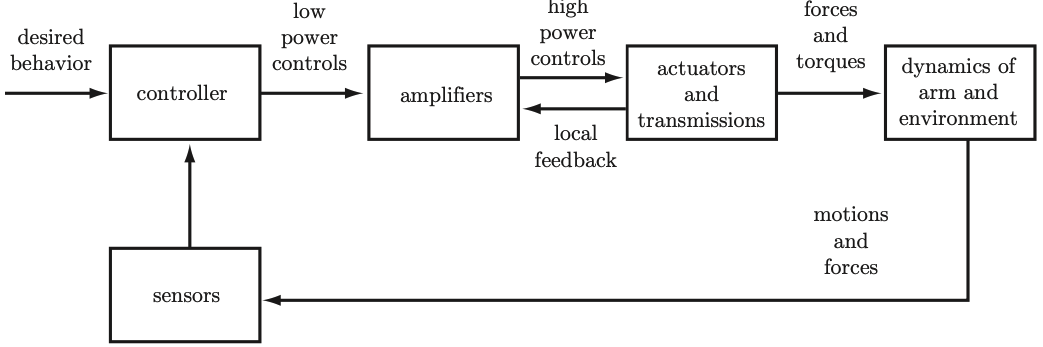
\includegraphics[scale=0.4]{control_diagram.png}
  \caption{A typical robot control system. An inner control loop is used to help the amplifier and actuator to achieve the desired force or torque [11].}
  \label{block_diagram}
\end{figure}
A remark needs to be done about the control of the translation of the base. It is highly improbable that it would be possibile to calculate the exact displacement of the spacecraft where the manipulator is attached, considering also the too little displacement from Figures~\ref{free_motion_1}, \ref{free_motion_2}. Hence, the control law is applied to $\theta_0, q_1$ and $q_2$ only. The base is free to move but, as already mentioned, it can be approximate as still, given the huge inertia of the spacecraft.\\ 
Thus, we can rewrite the final equation of motion (\ref{final_equation_motion}):
\begin{equation}
  \begin{bmatrix}
    M'_{tt}&M'_{tr}\\
    M'_{rt}&M'_{rr}
  \end{bmatrix}
  \begin{bmatrix}
    \ddot{p}_t\\
    \ddot{p}_r
  \end{bmatrix}+\begin{bmatrix}
    C'_{t}\\
    C'_{r}
  \end{bmatrix}=\begin{bmatrix}
    \textbf{0}\\
      u
    \end{bmatrix}
    \label{one_control}
\end{equation}
where $p_t=\{x_b,y_b\}$ refers to the translational coordinates, $p_r=\{\theta_0,q_1,q_2\}$ to the rotational ones and $\textbf{0}\in \mathbb{R}^2$.\\
By writing the translational coordinate as a function of the rotational ones
\begin{equation}
  \ddot{p}_t=-M_{tt}^{-1'}(M'_{tr}\ddot{p}_r+C'_t)
\end{equation}
and by plugging it in the second row of (\ref{one_control}):
\begin{equation}
  \ddot{p}_r\tilde{M}+\tilde{C}=u
  \label{rotation_equation_motion}
\end{equation}
with
\begin{equation}
\begin{array}{c}
  \tilde{M}=M_{rr}'-M_{rt}'{M'}_{tt}^{-1}M_{tr}', \quad \tilde{C}=C_r'-M_{rt}'{M'}_{tt}^{-1}C'_t
\end{array}
\end{equation}
If we knew perfectly the robot dynamics, we could use the following input (\textit{feed-forward}) to move the robot:
\begin{equation}
  \hat{u}=\hat{M}\ddot{q}_d+\hat{C}(q_d,\dot{q}_d)
\end{equation}
where the RHS of the equation is the estimaed robot dynamics.\\
Upon substitution in (\ref{rotation_equation_motion}), we would have, supposing $\hat{M}=\tilde{M}$ and $\hat{C}=\tilde{C}$:
\begin{equation}
  \tilde{M}(\ddot{q}_d-\ddot{q})=0
\end{equation}
which is true when the desired configuration is reached.\\
Since in practice it is not possible to know the exact dynamics, a PD controller is often used in addition to the feed-forward term to compensate for inaccuracy and disturbances:
\begin{equation}
  u=\hat{u}+K_p(q_d-q)+K_d(\dot{q}_d-\dot{q})
\end{equation}
with $K_p$ and $K_d$ the proportional and derivative positive definite gain matrices.\\
Assuming then $\hat{M}\approx\tilde{M}$ and $\hat{C}\approx\tilde{C}$ and substituting in (\ref{rotation_equation_motion}):
\begin{equation}
  \tilde{M}(\ddot{q}_d-\ddot{q})+K_d(\dot{q}_d-\dot{q})+K_p(q_d-q)=0
\end{equation}
However, the above equation is coupled by the mass matrix. In order to have an uncoupled control scheme, a \textit{feedback linearization} can be implemented, as suggested by [16]:
\begin{equation}
  u=\hat{M}[\ddot{q}_d+K_d(\dot{q}_d-\dot{q})+K_p(q_d-q)]+\hat{C}
  \label{feedback_linearization}
\end{equation}
such that the final equation of motion for the rotational coordinates becomes:
\begin{equation}
  \ddot{e}+K_d\dot{e}+K_pe=0
  \label{controlled_dynamics}
\end{equation}
The tracking error $e$ is governed by a second order dynamics that can be arbitrarily assigned (on each joint) by suitably selecting gains ($K_p,K_d$).\\
The dynamics is now:
\begin{itemize}
  \item decoupled: each joint coordinate evolves indipendently from others $\Rightarrow$ $K_p,K_d$ are diagonal matrices.
  \item linear: we have global asymptothic ($e\rightarrow 0$) stability for any $K_p\succ 0,K_d\succ 0$. This is a sufficient and necessary condition since the state-space equation is given by:
    \begin{equation}
      x=\begin{bmatrix}
        e\\\dot{e}
      \end{bmatrix}\quad \Rightarrow \quad \dot{x}=\begin{bmatrix}
        \mathbf{0}&I_{2\times 2}\\
        -K_p&-K_d
      \end{bmatrix}
    \end{equation}
    and, for second order differential equations, if $K_{p_i}>0$ and $K_{d_i}>0$, the dynamics is stable [11].
  \item the time evolution is governed by the eigenvalues that are the roots of the polynomial:
    \begin{equation}
      s^2+K_{d_i}s+K_{p_i}=0 \quad \Rightarrow \quad s_{1,2}=\frac{-K_{d_i}\pm \sqrt{K_{d_i}^2-4K_{p_i}}}{2}
    \end{equation}
    with $\omega_n=\sqrt{K_{p_i}}$ and $\xi=\frac{K_{d_i}}{2\sqrt{K_{p_i}}}$.
\end{itemize}

The control law shown in equation (\ref{feedback_linearization}) has been chosen with zero desired velocities $\dot{p}_d$ and with the initial positions (Table~\ref{initial_positions}) as desired coordinates $p_d$.\\
$K_p$ has been chosen as the identity matrix (i.e. $I_{5\times 5}$) and $K_d$ has been calculated following the relation of the damping term shown above and chosing a critically damped behaviour, so that there are no overshoots of the links while reaching the desired position:
\begin{equation}
  \xi=1 \quad \Rightarrow \quad K_d=2\sqrt{K_p}
  \label{critically_damped}
\end{equation}
The final results are shown in Figures~\ref{controlled_motion_1}, \ref{controlled_motion_2}, where underdamped and overdamped behaviours have been plotted as well.
\begin{figure}
  \centering
  \subfloat
  {\includesvg[scale=0.37]{controlled_motion_x.svg}}\quad
\subfloat
  {\includesvg[scale=0.37]{controlled_motion_y.svg}} \\
  \subfloat
  {\includesvg[scale=0.37]{controlled_motion_theta.svg}}\quad
  \subfloat
  {\includesvg[scale=0.37]{controlled_motion_q1.svg}
  \label{q1_real}}\\
  \subfloat
  {\includesvg[scale=0.37]{controlled_motion_q2.svg}}
  \caption{VMS generalized coordinates' displacement after the catching of the payload when no control is performed, simulation one. In yellow, an underdamped behaviour ($\xi=0.5$), in blue a critically damped behaviour ($\xi=1$), in green an overdamped behaviour ($\xi=1.5$).}
  \label{controlled_motion_1}
\end{figure}
\begin{figure}
  \centering
  \subfloat
  {\includesvg[scale=0.37]{controlled_motion_x2.svg}}\quad
\subfloat
  {\includesvg[scale=0.37]{controlled_motion_y2.svg}} \\
  \subfloat
  {\includesvg[scale=0.37]{controlled_motion_theta2.svg}}\quad
  \subfloat
  {\includesvg[scale=0.37]{controlled_motion_q12.svg}}\\
  \subfloat
  {\includesvg[scale=0.37]{controlled_motion_q22.svg}}
  \caption{VMS generalized coordinates' displacement after the catching of the payload when no control is performed, simulation two.}
  \label{controlled_motion_2}
\end{figure}
\newpage
\section{Elastic Bodies}
In this section, a more realistic scenatio is developed and the assumption of rigid bodies will be discarded: the links of the manipulator will be considered flexible.\\
The robotic systems with flexible links are continuous dynamical systems characterized by an infinite number of degrees of freedom and are governed by nonlinear, coupled, ordinary, and partial differential equations. The exact solution of such a mathematical model is normally not feasible, and the infinite dimensional model imposes severe constraint on the design of controllers as well. Hence it is necessary that these continuous systems are discretized. \\
Flexible links with rigid joints in robot manipulators are discretized by using assumed modes, finite elements, or lumped parameters. The link deflections, with respect to the link’s rigid configuration, are usually assumed to be small, and a linear theory of elasticity is selected. Researchers commonly utilize the Euler-Bernoulli beam theory to represent the dynamics of link flexibility, which is the one selected for this work [17].\\
The lateral vibration of a beam can be studied by considering it as a continuous system, characterized by an infinite number of degrees of freedom. The equation of motion is carried out by considering the forces and moments acting on an infinitesimal piece of the body (Figure~\ref{elementary}), whose mass can be written as:
\begin{equation}
\,dm=\rho Adx
\end{equation}
where $\rho$ is the beam densit and $A$ its cross-section area, whcih is considered constant along the beam.\\
\begin{figure}[h]
\centering
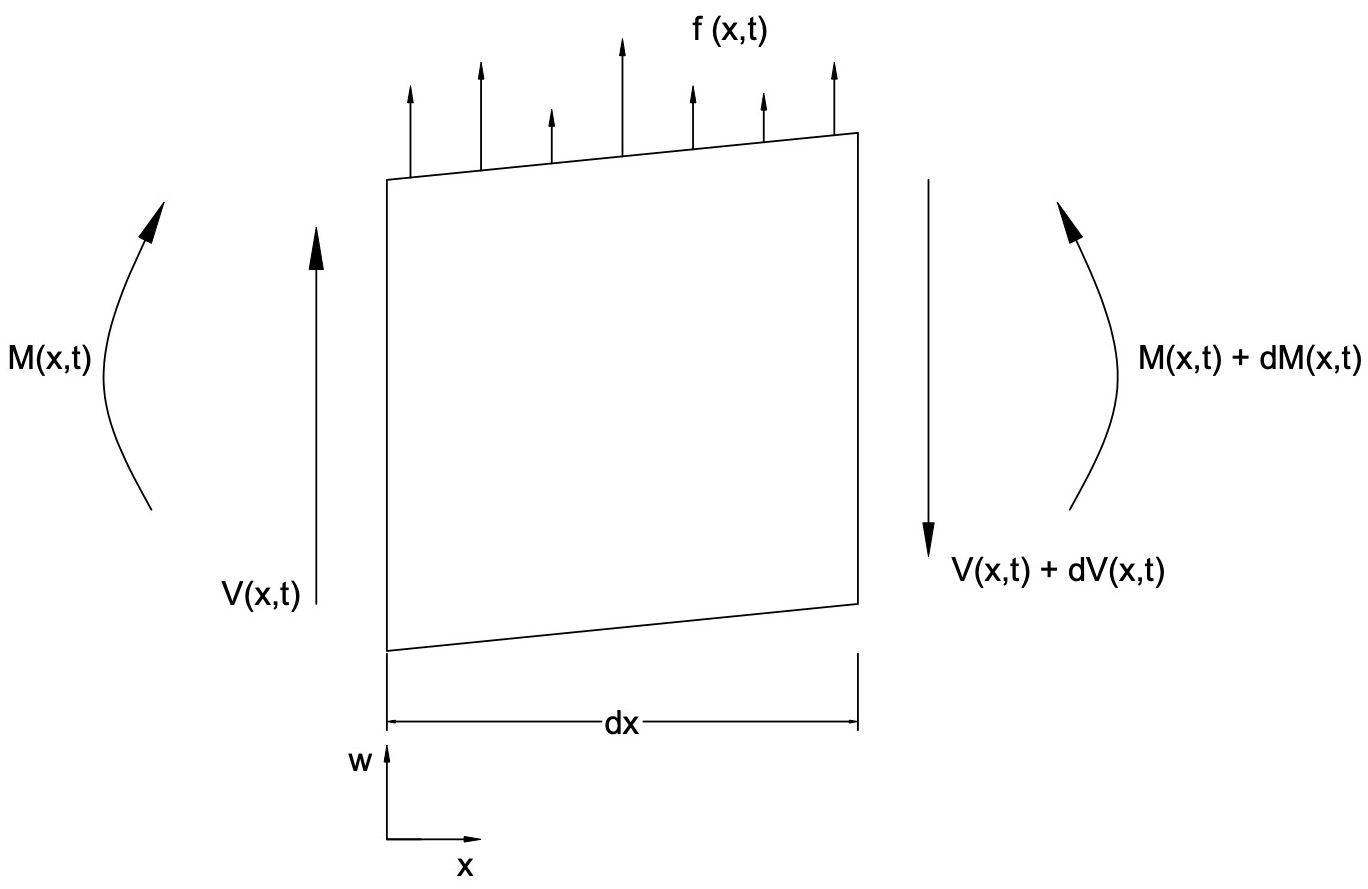
\includegraphics[scale=0.25]{elementary}
\caption{Forces acting on the infinitesimal piece of the beam.}
\label{elementary}
\end{figure}
The equations of motion are:
\begin{equation}
\begin{cases}
f(x,t)dx-(V+dV)+V=\rho A \,dx \frac{\partial^2w(x,t)}{\partial t^2}\\
(M+dM)-(V+\,dV)dx+f(x,t)dx\frac{dx}{2}-M=0
\end{cases}
\end{equation}
where $V$ is the shear force, $M$ the bending moment and $f(x,t)$ the distributed force. The dominant motion is assumed to be the lateral one, which is true when the beam is thin.\\
By defining $\,dV=\frac{\partial V}{\partial x}\,dx$ and $\,dM=\frac{\partial M}{\partial x}\,dx$, and using the Euler-Bernoulli definition of moment $M(x,t)=ES\frac{\partial^2 w(x,t)}{\partial x^2}$, where $E$ is the Young's modulus and $S$ is the area moment of inertia (not to be confused with the mass moment of inertia $I$), the equation of motion becomes:
\begin{equation}
  ES\frac{\partial^4w(x,t)}{\partial x^4}+\rho A\frac{\partial^2w(x,t)}{\partial t^2}=f(x,t)
\end{equation}
and, by defining $c=\sqrt{\frac{EI}{\rho A}}$ as the speed of longitudinal deformation, we get:
\begin{equation}
c^2\frac{\partial^4w(x,t)}{\partial x^4}+\frac{\partial^2w(x,t)}{\partial t^2}=f(x,t)
\label{forced}
\end{equation}
$EI$ can also be referred to \textit{flexural rigidity} of the beam.\\
The free vibration equation is obtained by imposing $f(x,t)=0$:\\
 \begin{equation}
c^2\frac{\partial^4w(x,t)}{\partial x^4}+\frac{\partial^2w(x,t)}{\partial t^2}=0
\label{free}
\end{equation}
which is also reported in [18]: we assume that no control is applied to the tips' deformations. This assumption will be tackled in the next sections.\\
The solution of the equation (\ref{free}) needs two initial condition and four boundary condition to be found. It can be calculated by separation of variables, writing the solution as the product of a function depending on time and another one depending on space:
\begin{equation}
w(x,t)=W(x)Q(t)
\label{separability}
\end{equation}
It is now possible to rewrite the equation (\ref{free}) as:
\begin{equation}
\frac{c^2}{W(x)}\frac{\,d^4W(x)}{\,dx^4}=-\frac{1}{Q(t)}\frac{\,d^2Q(t)}{\,dt^2}=const
\end{equation}
and by choosing as the constant $\omega^2$, the time equation becomes the one degree of freedom oscillator, whose solution is known (\ref{time}), while the space equation solution can be written as (\ref{space}), where $\beta^4=\frac{\rho A}{EI}\omega^2$.
\begin{equation}
Q(t)=A\cos{\omega t}+B\sin{\omega t}
\label{time}
\end{equation}
\begin{equation}
W(x)=c_1\cos(\beta x)+c_2\sin{\beta x}+c_3\cosh{\beta x}+c_4\sinh{\beta x}
\label{space}
\end{equation}
The four coefficient of the space solution can be found with the boundary condition of the system. Every natural frequency of the system is associated to one space solution (mode shape) and time solution, and can be found imposing the boundary conditions.\\
The displacement of the beam is the sum of the product between the $n$ mode shapes selected and their time solutions [16,17,18]:
\begin{equation}
w(x,t)=\sum_{n=1}^\infty W_n(x)Q_n(t)
\label{overall}
\end{equation}
As already mentioned, the assumption for the Euler-Bernoulli beams model is of small deformartions. The kinematic analysis can be carried out in the same way we did in Section~\ref{planar_VMS}, with the only addiction of homogeneous elasticity matrix, which accounts for the elastic deformation of the link [17]. Assuming null rotation and small tip deformation, we can write the elasticity matrix from link $i$ to $i+1$ as:
\begin{equation}
  \prescript{i}{i+1}{E}=\begin{bmatrix}
    1&0&0&u(x,t)\\
    0&1&0&w(x,t)\\
    0&0&1&v(x,t)
  \end{bmatrix}
\end{equation}
with $u(x,t),w(x,t),v(x,t)$ elastic deformations in the $x,y,z$ direction respectively.\\
Since the deformation is calculated at the arm's tip and only in the y-direction (following the Denavit-Hartenberg notation), we can rewrite the matrix:
\begin{equation}
  \prescript{i}{i+1}{E}=\begin{bmatrix}
    1&0&0&0\\
    0&1&0&W_i(x)Q_i(t)\\
    0&0&1&0
  \end{bmatrix}
\end{equation}
where $W_i(x)=\{W_{i,1},W_{i,2},\dots,W_{i,n}\}$ and $Q_i(t)=\{Q_{i,1},Q_{i,2},\dots,Q_{i,n}\}^T$ [16].\\
The joints' homogeneous transformation matrices, for the analyzed planar case, will be given as:
\begin{equation}
  \begin{array}{l}
  \prescript{f}{1}{T}=\prescript{f}{b}{M}\prescript{b}{0}{M}\prescript{0}{1}{M}\prescript{0}{1}{E}\\
  \prescript{f}{2}{T}=\prescript{f}{b}{M}\prescript{b}{0}{M}\prescript{0}{1}{M}\prescript{0}{1}{E}\prescript{1}{2}{M}\prescript{1}{2}{E}\\
  \end{array}
  \label{new_kinematics}
\end{equation}
Hence, the time-varying part of the free-vibration solution $Q(t)$ can be found by sollowing the lagrangian approach as in the previous sections, where the genetalized coordinate vector of the system is now:
\begin{equation}
  p=\{x_b,y_b,\theta_b,q_1,q_2,Q_1,Q_2\}
  \label{new_coordinates}
\end{equation}
and its dimension depends on the number of modeshapes chosen (e.g. for $n=1$, $p\in\mathbb{R}^7$).\\

For what regards the space-varying part of the free vibration solution $W(x)$, four boundary conditions need to be imposed. It is reasonable to suppose that the inertia of a lightweight link is small compared to the hub inertia, and then constrained mode shapes can be used. In particular, we assume each link to be clamped at the base:
\begin{equation}
  w_i(0,t)=0, \quad w_i'(0,t)=0
\end{equation} 
Furthermore, experiments and recent analytical studies have shown that the clamped assumption is even enforced when chosing a feedback control loop around the joint [18].\\
Concerning the remaining boundary conditions, we consider mass boundary conditions representing balance of moment and shearing force owing to other links of the serial structure of robot manipulators and the payload [17, 18]:
\begin{equation}
  \begin{array}{c}
  (EI)_i\frac{\partial^2w_i(l_i,t)}{\partial x^2}=-J_{L_i}\frac{d^2}{dt^2}\Big(\frac{\partial w_i(l_i,t)}{\partial x}\Big)-M_{D_i}\frac{d^2}{dt^2}w_i(l_i,t)\\
  (EI)_i\frac{\partial^3w_i(l_i,t)}{\partial x^3}=-M_{L_i}\frac{d^2}{dt^2}w_i(l_i,t)+M_{D_i}\frac{d^2}{dt^2}\frac{\partial w_i(l_i,t)}{\partial x}
  \end{array}
  \label{boundary_conditions}
\end{equation}
where $M_{L_i}$, and $J_{L_i}$, are the actual mass and moment of inertia at the end of link~$i$. Moreover, $M_{D_i}$ accounts for the contributions of masses of distal links, i.e., noncollocated at the-end of link $i$, weighted by the relative distance from axis $y$, (shearing axis at the end of link $i$). Incidentally, these contributions are often not included in mode shape analyses: if the arm has only one link, $M_{L_i}$  and $J_{L_i}$ are directly the payload mass and inertia, while the additional terms on the right-hand side of (\ref{boundary_conditions}) vanish ($M_{D_i}=0$) only when the payload is balanced at the tip.\\ 
For the generic intermediate $i$th link in an open kinematic chain arrangement, instead, $M_{L_i}$ is the constant sum of all masses beyond link $i$, but $J_{L_i}$, and $M_{D_i}$, depend on the position of successive links. Thus, for exact mode shapes computation, these quantities should be updated as functions of the arm configuration; this may considerably increase the complexity of model derivation, beside overloading the computational burden of on-line execution. Therefore, some practical approximation leading to constant-although nonzero-boundary conditions at the link end might be in order. For instance, a convenient position is to set $M_{D_i}=0$ and compute $J_{L_i}$, for a fixed arm configuration.\\
In the case of a planar RR manipulator, like the one used in this thesis, we would have:
\begin{equation}
  \begin{array}{l}
    M_{L_1}=m_2+m_p\\
    J_{L_1}=I_{2,z}+I_{O,z}+m_Ol_2^2\\
    M_{D_1}=(m_2\frac{l_2}{2}+m_Ol_2)\cos{q_2}-\chi\sin{q_2}
  \end{array}
\end{equation}
where $\chi$ is a term of an order of magnitude smaller than the first one, hence can be negletted.\\
Notice that in the considered case of only two links, $J_{L_1}$ is a constant; for more than two links, $J_{L_1}$ will become a function of the generalized coordonate of link 3 and following ones.\\
On the other handm for link 2:
\begin{equation}
  \begin{array}{l}
    M_{L_2}=m_p\\
    J_{L_2}=I_{O,z}\\
    M_{D_2}=0
  \end{array}
\end{equation}
The varying of $M_{D_1}$ in time, since it depends on the arm configuration, implies that the mode shapes, which are spacial quantities, would become implicit function of time, thus conflicting with the original separability assumption (\ref{separability}).\\
However, $M_{D_1}$ can be rendered constant for a fixed arm configuration: assuming small displacement and initial position $q_{2,0}=\pi/2$, leads to $M_{D_1}=0$. That is why this has been chosen as the maniupaltor initial condition in both Section~\ref{rigid} and this one.\\
By substituting in the boundary conditions equations the solutions (\ref{time},\ref{space}), the homogeneous solution for link $i$ and mode shape $j$ is [17, 18]:
\begin{equation}
  W_{i,j}(x)=C_{i,j}[\cos{(\beta_{i,j} x)}-\cosh{(\beta_{i,j} x)}+\nu_i(\sin{(\beta_{i,j} x)}-\sinh{(\beta_{i,j} x)})]
  \label{lateral_solution}
\end{equation}
where:
\begin{equation}
  \nu_{i,j}=\frac{\sin{(\beta_{i,j}l_i)}-\sinh{(\beta_{i,j}l_i)}+M\beta_{i,j}[\cos{(\beta_{i,j}l_i)}-\cosh{(\beta_{i,j}l_i)}]}{\cos{(\beta_{i,j}l_i)}+\cosh{(\beta_{i,j}l_i)}-M\beta_{i,j}[\sin{(\beta_{i,j}l_i)}-\sinh{(\beta_{i,j}l_i)}]}
\end{equation}
where 
\begin{equation}
  M=\frac{M_L}{\rho A l}, \quad J=\frac{J_L}{\rho Al^3}
\end{equation}
and $\beta_{i,j}$ are solutions of the frequency equation:
\begin{equation}
  \begin{split}
  1+\cos{(\beta_{i,j}l_i)}\cosh{(\beta_{i,j}l_i)}&-M\beta_{i,j}[\cosh{(\beta_{i,j}l_i)}\sin{(\beta_{i,j}l_i)}-\sinh{(\beta_{i,j}l_i)}\cos{(\beta_{i,j}l_i)}]\\
  &-J\beta_{i,j}^3[\cosh{(\beta_{i,j}l_i)}\sin{(\beta_{i,j}l_i)}+\sinh{(\beta_{i,j}l_i)}\cos{(\beta_{i,j}l_i)}]\\
  &+MJ\beta^4[1-\cosh{(\beta_{i,j}l_i)}\cos{(\beta_{i,j}l_i)}]=0
  \end{split}
  \label{freq_equation}
\end{equation}
The remaining constant in equation (\ref{lateral_solution}) (i.e. $C_{i,j}$) is found by mass normalizing the mode shape:
\begin{equation}
  \int_{0}^{l_i}\rho_i A_i W_{i,j}^2(x)dx=1
\end{equation}
where the RHS of the equation is the modal mass of the $j$th mode of the $i$th link.\\
Mode shapes, in fact, can be normalized in different ways (normalization to the unit length vector, normalization to the largest component equal to unity), but the mass normalization is the most common one [19, 20], since it allows to have modal displacements with a physical meaning, since they are related to the modal mass.\\
The choice of the normalization, however, does not affect the value of the natural frequencies, which are the same for all the normalizations and depend only on equation (\ref{freq_equation}).\\

Once $W_{i,j}(x)$ are known, the kinematics can be evaluated through (\ref{new_kinematics}), and the dynamics can be calculated as in the previous sections, with the awareness that it is not possible to neglet the potential energy anymore.\\
If in the previus sections the absence of gravity and the rigidity of the bodies allowed to ignore it, now the maniupulators' arms are modeled as elastic bodies, thus the elastic potenatial energy needs to be taken into account.\\
The elastic energy for unit length stored in a bended beam can be written as [21]:
\begin{equation}
  \frac{dU}{dx}=\frac{1}{2}\frac{M^2}{ES}
  \label{partial_elastic}
\end{equation}
with $M$ torque moment, which can be expressed as:
\begin{equation}
  M=ES\kappa
  \label{torque_moment}
\end{equation}
where $\kappa$ is the curvature of the deformation, defined as the derivative of the deformation angle $\varphi$:
\begin{equation}
  \kappa=\frac{d\varphi}{dx}=\frac{d}{dx}\frac{\partial w(x,t)}{\partial x}=\frac{\partial^2 w(x,t)}{\partial x^2}
  \label{curvature}
\end{equation}
By substituting (\ref{curvature}) in (\ref{torque_moment}) and then in (\ref{partial_elastic}), by integration along the beam direction we get:
\begin{equation}
  \begin{split}
  U&=\frac{1}{2}\int_{0}^{l_i}ES\Big(\frac{\partial^2 w(x,t)}{\partial x^2}\Big)^2\,dx\\
   &=\frac{1}{2}\int_{0}^{l_i}ES\Big(\frac{\partial^2 W(x)}{\partial x^2}Q(t)\Big)^2\,dx
  \end{split}
\end{equation}
which is the same equation reported in [17, 18].\\
The new lagrangian will be now:
\begin{equation}
  \mathcal{L}_i = T_i-U_i
\end{equation}
and the dynamics of the system is given by:
\begin{equation}
  \begin{cases}
    \frac{d}{dt}\frac{\partial \mathcal{L} }{\partial \dot{x}_b}-\frac{\partial \mathcal{L} }{\partial x_b}=F_x\cos{\theta_0}-F_y\sin{\theta_0}\\
    \frac{d}{dt}\frac{\partial \mathcal{L} }{\partial \dot{y}_b}-\frac{\partial \mathcal{L} }{\partial y_b}=F_x\sin{\theta_0}+F_y\cos{\theta_0}\\
    \frac{d}{dt}\frac{\partial \mathcal{L} }{\partial \dot{\theta}_0}-\frac{\partial \mathcal{L} }{\partial \theta_0}=\tau_0\\
    \frac{d}{dt}\frac{\partial \mathcal{L} }{\partial \dot{q}_1}-\frac{\partial \mathcal{L} }{\partial q_1}=\tau_1\\
    \frac{d}{dt}\frac{\partial \mathcal{L} }{\partial \dot{q}_2}-\frac{\partial \mathcal{L} }{\partial q_2}=\tau_2\\
    \frac{d}{dt}\frac{\partial \mathcal{L} }{\partial \dot{Q}_1}-\frac{\partial \mathcal{L} }{\partial Q_1}=0\\
    \frac{d}{dt}\frac{\partial \mathcal{L} }{\partial \dot{Q}_2}-\frac{\partial \mathcal{L} }{\partial Q_2}=0
  \end{cases}
\end{equation}
since no torque is applied to control the vibrations at the arms' end.\\
We can directly find the stiffness matrix, of the system, without calculating from scratch the equations of motion, through the following considerations:
\begin{equation}
  \frac{d}{dt}\frac{\partial U}{\partial \dot{Q}_i}-\frac{\partial U}{\partial Q_i}=0+\int_{0}^{l_i}ES\frac{\partial^2 W(x)}{\partial x^2}\,dx
\end{equation}
Hence, as reported in [16], the new set of dynamical equation is obtained in the form:
\begin{equation}
  M\ddot{p}+C+Kp=u+J^Tf_I
\end{equation}
which is similar to the equation of motion of Chapter~\ref{impact_analysis} (\ref{initial_impact}), with the addiction of the stiffnes matrix $K=\operatorname{diag}(\textbf{0},K_1,K_2)$ where:
\begin{equation}
  K_i=\int_{0}^{l_i}E_iS_i\frac{\partial^2 W_i(x)}{\partial x^2}\,dx
\end{equation}
Following the same procedure shown in the previous Chapter and in Section~\ref{rigid}, under the assumption that during the impact no change in the VMS' positions happens (i.e. we can neglet matrix $K$ and follow the exact same calculus), the dynamic equation of the whole system VMS plus payload becomes [16]:
\begin{equation}
  M'\ddot{p}+C'+Kp=u
\end{equation}
similar to (\ref{VMS_dynamics}) and with $p$ as in (\ref{new_coordinates}).
\newpage
\subsection{Free Motion}
The frequency equation (\ref{freq_equation}) is a trascendental equation, so it has been solved with a finding-root algorithm (Mathematica provides it with a built-in command \texttt{FindRoot}), as shown in Figures~\ref{freq_plot_1} and \ref{freq_plot_2}.
A free motion simulation has been performed with the same initial condition and parameters of the previous section, adding the new ones exposed in Table~\ref{elastic_paramters}. The joints' evolution can be seen in Figure~\ref{free_elastic_1} and \ref{free_elastic_2}.
\chapter{Inertial and Kinetics Properties Retrieval}
In the previous chapter, the captured object has been considered as a deterministic disturbance, i.e. the inertia and dynamic properties have been supposed known.\\
However, in real case scenarios, the payload mass can be unknown (e.g. the captured of a small metoerite or of a satellite with estimated mass).\\
In this chapter, the same problem of payload docking will be anlysed supposing unknown mass, trying to retrive it from the manipulator post-impact dynamics together with its initial velocities, which are not known a priori.
\newpage
\section{Mass Extraction}
When the mass is not known, an estimate of the mass has to be injected in the control law (\ref{feedback_linearization}). This value can be estimated by visual techniques or thanks to previus knowledge.\\
Before starting to calculate the real mass, some approximations has to be taken into account:
\begin{itemize}
  \item the spacecraft does not move; this has already been shwon as a good approximation in the previous chapter
  \item the spacecraft does not rotate; this has also been shown in the previuos calculations (see Figures~\ref{controlled_motion_1}, \ref{controlled_motion_2})
  \item the displacement of one arm in the controlled dyanamics is negligible for the displacement of the other arm. From Figures~\ref{controlled_motion_1}, \ref{controlled_motion_2} it can be seen that also the arms displacement is little, so we can approximate them to zero when analyzing the other arm's dynamics
  \item given the little displacements after the impact, the mass and Coriolis' matrices can be linearized around the equilibrium position
\end{itemize}
With these suppositions, we can uncouple the dynamics of the two arms, since the accelerations and velocities of the all other coordinates are set to zero. We can furthermore set $C'=\hat{C'}$, since it depends on the coordinates positions and velocites.\\
Figure~\ref{approximations} shows two time evolutions of the displacement of both arms with and without applying the approximation made above. The behaviour is almost identical.\\
\begin{figure}
  \centering
  \subfloat[\emph{$q_1$ time evolution.}]
  {\includesvg[scale=0.4]{approximation_1.svg}} \\
\subfloat[\emph{$q_2$ time evolution.}]
  {\includesvg[scale=0.4]{approximation_2.svg}}
  \caption{Arms behaviours with estimated mass \SI{2000}{\kilogram}, with (orange) and without (blue) approximations for the first simulation.}
  \label{approximations}
\end{figure}
We can now rewrite the controlled dynamics (\ref{controlled_dynamics}) of the two arms as follows:
\begin{equation}
  \begin{array}{l}
    m_1\ddot{q}_1+\tilde{m_1}k_d\dot{e_1}+\tilde{m_1}k_p e_1=0\\
    m_2\ddot{q}_2+\tilde{m_2}k_d\dot{e_2}+\tilde{m_2}k_p e_2=0
  \end{array}
\end{equation}
Since the real mass is unknown, the approximation $M'=\hat{M'}$ is not possible anymore, that is why the supposed mass $\tilde{m}$ appears in the equation.\\
We can divide for $m_1$ and $m_2$ to get:
\begin{equation}
  \begin{array}{l}
    \ddot{q}_1+\frac{\tilde{m_1}}{m_1}k_d\dot{e}_1+\frac{\tilde{m_1}}{m_1}k_p e_1=0\\
    \ddot{q}_2+\frac{\tilde{m_2}}{m_2}k_d\dot{e}_2+\frac{\tilde{m_2}}{m_2}k_p e_2=0
  \end{array}
  \label{approx_dynamics}
\end{equation}
When the new control law with the estimated mass is applied, the behaviours is not criticaly damped anymore, since, as we can see from equations (\ref{approx_dynamics}): the new damping coefficient is now given by:
\begin{equation}
  \xi'=\frac{\tilde{m}k_v}{2\omega_n m}=\frac{\tilde{m}2\sqrt{k_p}}{2\sqrt{\frac{\tilde{m}}{m}k_p} m}=\sqrt{\frac{\tilde{m}}{m}}
  \label{mass_relation}
\end{equation}
\newpage
\subsection{Symbolic Approach}
Now that we have linear second order differential equations, like the ones in equation (\ref{approx_dynamics}), two methods have been introduced to retrieve the inertial properties of the payload (i.e. its mass). The first one, exposed in this section, is based on the fact that the solution of equations (\ref{approx_dynamics}) is known.\\
However, not only its solution is known in closed form, but it is possible to find the exact solution by solving directly the second order equation. Both approaches are exploited.
\subsubsection{Direct Solution}
Given the simplicity of the equation of motions, a direct symbolic solution, containing $\tilde{m}$ as a parameter, can be easily found (i.e. $q(t,\tilde{m})$).\\
Figure~\ref{parametric_plot} shows how the time response of the first joint for the first simulation changes according to the estimated mass. It is of particular interest the increasing of the first peak as the estimated mass increases.\\
\begin{figure}[!b]
  \centering
  \includesvg[scale=0.45]{parametric_plot.svg}
  \caption{Parametric plot of the first joint's time evolution, first simulation. The real mass is $\SI{3000}{\kilogram}$. A visual parameter setting can be possibile by confronting this plot with the real one (see Figure~\ref{q1_real}).}
  \label{parametric_plot}
\end{figure}
Hence, once the peak time $t*$ is found, the real mass can be calculated by solving the following equation:
\begin{equation}
  q(t*,\tilde{m})=q*
\end{equation}
with $q*$ the peak value.
\subsubsection{Closed Form Solution}
\paragraph{First Joint}
For the first joint, which has both initial position and velocity equal to zero, the equation of motion (\ref{approx_dynamics}) becomes:
\begin{equation}
  m_1 \ddot{q}_1+\tilde{m_1}k_d\dot{q}_1+\tilde{m_1}k_p q_1=0
\end{equation}
This can be threated as an homogeneous second order linear equation with one degree of freedeom.
Its solution is given by the well known formula:
\begin{equation}
  q_h(t)=\Big[q_0\cos{(\omega_d)t}+\frac{\dot{q}_0+\xi\omega_n q_0}{\omega_d}\sin{(\omega_dt)}\Big]e^{-\xi \omega_n t}
\end{equation}
where $q_0,\dot{q}_0$ are the initial position and velocity of the joint and $\omega_d=\sqrt{1-\xi^2}\omega_n$. Notice that $\dot{q}_0$ is now given by the velocity of the joint after the impact.\\
Given null initial position, we can further simplify the solution:
\begin{equation}
  q_h(t)=\frac{\dot{q}_0}{\omega_d}\sin{(\omega_dt)}e^{-\xi \omega_n t}
  \label{first_joint}
\end{equation}
It is easier to find a relationship between the real mass and the peak time by differentiating equation (\ref{first_joint}), so that the RHS term becomes zero:
\begin{equation}
  \sqrt{1-\xi^2}\cos{(\sqrt{1-\xi^2}\omega_nt*)-\xi\sin{(\sqrt{1-\xi^2\omega_nt*})}}=0
  \label{time_solution}
\end{equation}
which can be rearranged:
\begin{equation}
  \begin{array}{l}
  \tan{(\sqrt{1-\xi^2}\omega_nt*)}=\frac{\sqrt{1-\xi^2}}{\xi}\\
  \Rightarrow \tan{(\sqrt{1-\xi^2}\omega_nt*)}=\beta(\xi)
\end{array}
\end{equation}
The intersection of the two functions allows to calculate the damping coefficient of the equation and thus the real mass from relation (\ref{mass_relation}).
\paragraph{Second Joint}
The equation of motion of the second joint, on the other hand, is:
\begin{equation}
  m_2\ddot{q}_2+\tilde{m_2}k_d\dot{q}_1+\tilde{m_2}k_p (q_2-q_{2,d})=0
\end{equation}
Now the desired position, which is the initial one, is not zero anymore. However, by moving the term on the RHS of the equation, we get a forced differential equation with constant external input:
\begin{equation}
  m_2\ddot{q}_2+\tilde{m_2}k_d\dot{q}_1+\tilde{m_2}k_p q_2=\tilde{m_2}k_pq_{2,d}
  \label{new_q2}
\end{equation}
Equation (\ref{new_q2}) can be considered as a system subjected to a step function of amplitude $F_0=\tilde{m_2}k_pq_{2,d}$. The particular solution of such system is also known:
\begin{equation}
  \begin{split}
  q_f(t)&=\frac{F_0}{k}\Big[1-\frac{e^{-\xi\omega_nt}}{\sqrt{1-\xi^2}}\sin{(\omega_dt+\theta)}\Big]\\
  &=q_{2,d}\Big[1-\frac{e^{-\xi\omega_nt}}{\sqrt{1-\xi^2}}\sin{(\omega_dt+\theta)}\Big]
\end{split}
\end{equation}
with $\theta=\arccos{\xi}$ and $k=\tilde{m_2}k_p$ elastic coefficient.\\
The total solution will be given by the sum of the homogeneous and the particular solution:
\begin{equation}
  q_2(t)=q_{2,d}\Big[1-\frac{e^{-\xi\omega_nt}}{\sqrt{1-\xi^2}}\sin{(\omega_dt+\theta)}\Big]+\Big[q_0\cos{(\omega_d)t}+\frac{\dot{q}_0+\xi\omega_n q_0}{\omega_d}\sin{(\omega_dt)}\Big]e^{-\xi \omega_n t}
\end{equation}
By differentization of the above equation, one gets:
\begin{equation}
  \begin{array}{c}
  \begin{tiny}
  \frac{e^{-\xi \omega t}\{2 \dot{q}_0 [\sqrt{1-\xi^2} \cos (\omega_dt)-\xi \sin (\omega_dt)]-(\pi -2 q_0) \omega [\xi \sqrt{1-\xi^2} \cos (\omega_dt)-(\xi^2-1) \sin (\omega_dt)]\}}{2 \sqrt{1-\xi^2}}=0
\end{tiny}
\end{array}
\end{equation}
but since the initial position $q_{2,0}=\pi/2$, the second term becomes zero and we end up with equation (\ref{time_solution}) again. Hence, the same procedure holds.
\newpage
\subsection{Interpolation Approach}
\end{document}
